\documentclass[a4paper,12 pt]{report}

\usepackage[T1]{fontenc}
\usepackage[polish]{babel}
\usepackage[margin=1in]{geometry}
\linespread{1.3}
\usepackage[utf8]{inputenc}
\usepackage{lmodern}
\usepackage{amsmath}
\usepackage{graphicx}
\usepackage{makeidx}
\usepackage{caption}
\usepackage{placeins}
\usepackage{listings}
\usepackage{xcolor}
\usepackage{gb4e}

\lstset {
    language=C++,
    frame=tb,
    tabsize=4,
    showstringspaces=false,
    numbers=left,
    %upquote=true,
    commentstyle=\color{commentgreen},
    keywordstyle=\color{brown},
    stringstyle=\color{red},
    basicstyle=\small\ttfamily, % basic font setting
    emph={int,char,double,float,unsigned,void,bool},
    emphstyle={\color{blue}},
    escapechar=\&,
    % keyword highlighting
    classoffset=1, % starting new class
    otherkeywords={>,<,.,;,-,!,=,~},
    morekeywords={>,<,.,;,-,!,=,~},
    keywordstyle=\color{orange},
    classoffset=0,
}

\noautomath

 \setcounter{tocdepth}{4}
 \setcounter{secnumdepth}{4}
 
\DeclareCaptionType{mycapequ}[][List of equations]
\captionsetup[mycapequ]{labelformat=empty}


\makeatletter
\setlength{\@fptop}{0pt}


\makeindex
\selectlanguage{polish}


\newcommand{\linia}{\rule{\linewidth}{0.4mm}}
\renewcommand{\maketitle}{\begin{titlepage}
    \vspace*{1cm}
    \begin{center}\small
   \textbf{ Rafał Cieślak}\\
    nr albumu : 34203\\
    kierunek studiów: Informatyka\\
    specjalność: Systemy komputerowe i opramowanie\\
    forma studiów: stacjonarne
    \end{center}
    \vspace{3cm}
    \noindent\linia
    \begin{center}
      \textbf{ \textsc{\@title}}
         \end{center}
     \linia
    \vspace{0.5cm}
    \begin{flushright}

    \vspace{5cm}
        \begin{center}\small
     {\small Praca dyplomowa inżynierska wykonana pod przewodnictwem:}\\
         dr inż. Tomasz Mąka
             \end{center}
     \end{flushright}
    \vspace*{\stretch{6}}
    \begin{center}
   Szczecin 2019
    \end{center}
  \end{titlepage}%
}
\makeatother
\title{Identyfikacja akustyczna rodzaju zdania w systemach dialogowych	\newline \newline Acoustic identification of sentence type in dialogue systems	}
\begin{document}
\maketitle




\newpage
\tableofcontents
\listoffigures



\newpage
\begin{abstract}
   Niniejsza praca inżynierska dotyczy analizy przebiegu intonacji w zdaniach wypowiedzianych w języku polskim. Omówione zostały zagadnienia związane z wytwarzaniem mowy, częstotliwością podstawową oraz funkcjami intonacji. Celem pracy było zaobserwowanie charakterystycznych cech, towarzyszących każdemu z rodzajów wypowiedzi. W ramach pracy sporządzono bazę 90 nagrań, których intonacja była poddawana analizie wizualnej. Na podstawie tych obserwacji zaimplementowany został program, dokonujący klasyfikacji wypowiedzi. Do esktrakcji intonacji użyty został algorytm YIN. W ramach pracy porównano również skuteczność zaproponowanej metody klasyfikacji dla wartości intonacji uzyskanych za pomocą programu PRAAT.
  \vskip.5\baselineskip
 
 \centerline{\bfseries Abstract}
 This engineering thesis concerns analysis of intonation in utterances spoken in Polish. Among discussed topics there were ones related to speech production, fundamental frequency and functions of intonation.The purpose of this thesis was to observe the characteristic features that accompany various types of utterance. As part of a work, a database of 90 recordings was prepared. Their intonation was analysed. Basing on these observations, the classifying program has been implemented.The YIN algorithm was used as a way to isolate the intonation.As part of the work, a comparison was made between the classification results obtained using the proposed method, for intonation isolated by YIN and PRAAT.
 \vskip.5\baselineskip\rmfamily

 

\end{abstract}
\newpage
\section*{Wstęp}
\addcontentsline{toc}{section}{Wstęp}
Mowa jest najpowszechniejszym sposobem komunikacji międzyludzkiej. Używając jej na codzień, nie zdajemy sobie sprawy jak bardzo złożonym jest procesem. Wydaje się być czymś normalnym i oczywistym. Mimo tego, że otacza nas cały czas, nauka wciąż nie poznała dokładnie wszystkich mechanizmów stojących za jej wytwarzaniem i rozumieniem. Złożoności dodaje fakt, że w mowie nie chodzi tylko o wypowiedziane słowa. Dla naszego odbierania mowy ważna jest również cała otoczka - ton głosu, jego barwa, akcentowanie i wiele więcej cech, których postrzeganie jest subiektywne. Dawno zostało zauważone, że cechy te mogą istotnie wpływać na nasze życie. Ludzie podświadomie wybierają towarzystwo osób, których głos jest dobrze przez nich postrzegany. Bez tych otaczających wypowiadane słowa cech, nasza mowa brzmiałaby podobnie do uzyskiwanej za pomocą syntezatorów.

Jedną z takich cech jest intonacja. Przy tym jest jednym ze słabiej poznanych zagadnień związanych z wytwarzaniem oraz percepcją mowy. Nie niesie ze sobą żadnej semantycznej treści, dotyczy tego w jaki sposób coś mówimy, a nie co mówimy. Nie zdajemy sobie na codzień z tego sprawy ale bez niej bardzo trudne byłoby zrozumienie języka mówionego i przekazywanych za jego pomocą myśli. Wpływa na nasze postrzeganie zdań wypowiedzianych przez naszego rozmówcę. Dzięki niej momentalnie wiemy czy osoba, z którą rozmawiamy zadała nam pytanie czy nakazała nam wykonanie jakiejś czynności. Nie potrzebujemy do tego znaków przestankowych, używanych w języku pisanym.

Celem pracy jest zrozumienie jak bardzo wpływa na ten proces i odpowiedź na pytanie czy analizowanie samej intonacji jest wystarczające do stwierdzenia do jakiej kategorii można zakwalifikować daną wypowiedź. W tym celu podjęta została próba wykrycia charakterystycznych cech intonacji, związanych z różnymi typami wypowiedzi, których zastosowanie umożliwi automatyczne klasyfikowanie zdań przez program.

Jako, że analiza będzie się opierać w głównej mierze na próbach zauważenia charakterystycznych róznic między róznymi wypowiedziami, metodą badawczą zastosowaną w tej pracy będzie metoda obserwacyjna.

Praca została podzielona na trzy główne rozdziały.
W rozdziale pierwszym przedstawione zostały istotne zagadnienia teoretyczne związane z produkcją mowy, wytwarzaniem częstotliwości podstawowej,
oraz przybliżone zostały funkcje intonacji. W rozdziale drugim omówiony został sposób implementacji wykrywania poszczególnych segmentów w przebiegu całej intonacji. W rozdziale trzecim przedstawione zostały rezultaty analizy charakterystycznych cech dla poszczególnych rodzajów wypowiedzi.
\newpage
\chapter{Wprowadzenie teoretyczne}

\section{Sygnał mowy}
Mową okreslamy komunikowanie się między sobą ludzi, za pomocą ukształtowanego zbioru dźwięków i reguł, zwanego językiem. Każdy język używa własnych fonetycznych kombinacji zbioru spółgłosek i samogłosek, które tworzą słowa mające semantyczne znaczenie. W czasie mówienia, osoba mówiąca poza samym wypowiadaniem słów, nadaje wypowiedzi znaczenie również za pomocą dodatkowych aspektów, takich jak intonacja, tempo mówienia czy stopień głosnosci.
Sama produkcja mowy jest wielokrokowym procesem zamiany myśli w ustną wypowiedź, która może być zarejestrowana jako sygnał mowy.


 
\subsection{Powstawanie mowy}

Sygnal mowy ludzkiej jest sygnałem akustycznym powstającym podczas przepływu powietrza poprzez aparat mowy, który jest definiowany jako 3 osobne grupy narządów~\cite{speech}.

Składowymi aparatu mowy są:
\begin{enumerate}
\item Aparat oddechowy. Bierze udział w początkowej fazie powstawania mowy, dostarczając kolejnym składowym strumień powietrza, który jest niezbędny do wygenerowania drgań. Dzieje się to podczas wydechu. Elementy, z których jest zbudowany to płuca, oskrzela, przepona oraz tchawica.

\item Aparat fonacyjny, którego głównym elementem jest krtań. Jest to narząd niezbędny do wygenerowania jakiegokolwiek dźwięku, nie tylko mowy. Najważniejszym elementem krtani, w kontekście procesu powtarzania dźwięku, są fałdy głosowe. W ich skład wchodzą więzadła głosowe oraz mięśnie głosowe. Przestrzeń pomiędzy nimi nazywana jest szparą głośni. Struktury te przybliżają się i oddalają od siebie podczas powstawania dźwięku co powoduje zwarcie i rozwarcie szpary głośni. Podczas oddychania oraz przy generowaniu głosek bezdźwięcznych, fałdy są rozsunięte, natomiast zwierają się  i rozwierają podczas powstawania głosek dźwięcznych. 
Dzięki tej czynności, strumień powietrza wprowadzany jest w drgania, co postrzegamy jako dźwięczność. Cecha ta występuje wraz z każdą samogłoską oraz przy niektórych spółgłoskach. Podczas drgań generowany jest ton krtaniowy, zwany również częstotliwością podstawową, oznaczany w literaturze jako F0. 
\begin{figure}[!htbp]

\centering
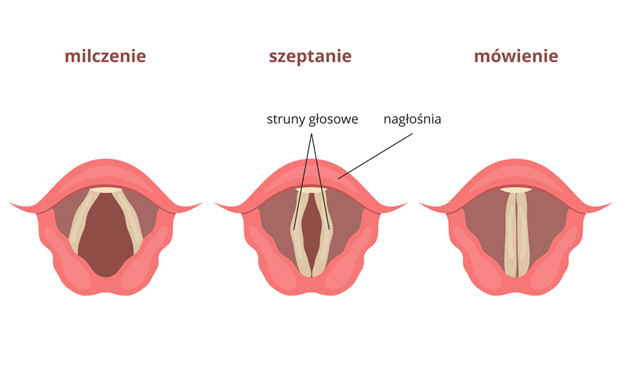
\includegraphics[scale=0.5]{faldy_glosowe}
\caption{Fałdy głosowe ~\cite{krtan}}

\end{figure}
\FloatBarrier


\item Aparat artykulacyjny, w którego skład wchodzą jamy przewodu oddechowego, znajdującego się ponad krtanią. Najważniejsze z punktu widzenia artykulacji - nosowa, gardłowa oraz ustna - nazywane są nasadą. Artykulatory znajdujące się w nasadzie dzielone są na ruchome oraz nieruchome. Do ruchomych zaliczamy język, podniebienie miękkie, wargi oraz żuchwę. Nieruchomymi określamy zęby, dziąsła oraz podniebienie twarde. Ich ustawienie ostatecznie determinuje cechy wytwarzanego dźwięku. 
\end{enumerate}
 W zaleźnosci od tego czy dana głoska jest dźwięczna czy bezdźwięczna proces powstawania dźwięku przebiega w trochę inny sposób. W obu przypadkach w początkowej fazie wzrasta cisnienie w płucach, co prowadzi do wydechu~\cite{produkcja_mowy}. Powietrze dostaje się do tchawicy. Na szczycie tchawicy znajduje się krtań, należąca do aparatu fonacyjnego. W przypadku głosek dźwięcznych, w miarę przepływu powietrza przez głosnię, spada lokalne cisnienie, co pozwala mięsniom krtani zamknąć głosnię, przerywając przepływ powietrza. To powoduje wzrost cisnienia, prowadzący do kolejnego oddalenia się strun głosowych. Cały ten cykl zapętla się, struny wibrują tworząc dźwięk, kierowany do aparatu artykulacyjnego. Na tym etapie, poza artykulacją, zachodzi również tłumienie niektórych częstotliwosci, nie będących harmonicznymi fali głosniowej. Nie wytłumione zostają tylko częstotliwosci będace bliskie naturalnemu rezonansowi traktu głosowego. Ruszając szczęką, ustami lub zmieniając połozenie języka, możemy zmieniać uzyskiwany dźwięk, ponieważ zmieni się rezonans traktu głosowego, a zatem inne częstotliwosci zostaną wytłumione. Gdy wypowiadane są głoski bezdźwięczne, krtań nie odgrywa istotnej roli, a modulacja dźwięku odpowiedzialna za uzyskanie brzmienia głoski odbywa się w aparacie artykulacyjnym. Jako rezultat kompletnego procesu, uzyskiwana jest fala akustyczna, wydostająca się z ust. Prawdziwosć opisanych różnic między dwoma rodzajami głosek można sprawdzić w prosty sposób, przykładając palce do krtani. W czasie wypowiadania głosek dźwięcznych czyli wszystkich samogłosek oraz częsci spółgłosek, takich jak b, d, g, w, z, ź, ż, l, ł, r, m, n, j , dz, dź, dż, wyczuwalne będę wibracje, które nie wystąpią podczas wypowiadania głosek bezdźwięcznych, takich jak p, t, k, f, s, ś, sz, c, ć, cz, ch.
Fakt, że wiele różnych narządów bierze udział w tworzeniu mowy powoduje, że zaburzenia zdrowotne każdego z nich mają istotny wpływ na cały proces. Zakres powstałych w ten sposób zaburzeń mowy jest szeroki - od drobnych wad wymowy do całkowitej utraty mowy.



\subsection{Reprezentacja mowy}
W procesie rozwoju technologii związanych z  przetwarzaniem mowy, konieczne bylo ustalenie sposobu przedstawienia wypowiedzi za pomocą symboli reprezentujacych wyprodukowany sygnal. Litery, używane w tym celu w języku pisanym, są niewystarczające, ponieważ w różnych wyrazach mogą być wymawiane na rózne sposoby.  Często produkowany dźwięk dla danej litery różni się w zależnosci od otaczających ją liter. Dla języka polskiego charakterystyczne jest występowanie tak zwanych dwuznaków, na przykład ''rz,sz,ch''. Dźwięk produkowany dla tych znaków jest calkowicie odmienny od dźwięków reprezentujących każdą z liter osobno. 
Jednym ze sposobów reprezentowanie dźwięków powszechnie występujących w danym języku są fonemy. Są to najmniejsze elementy języka mówionego, pozwalające na rozróżnienie poszczególnych słów~\cite{phonem}. Często po zamienieniu jednego z fonemów składowych na inny, znaczenie słowa może ulec zmianie. W lingwistyce istnieją rózne sposoby definiowania czym są fonemy oraz w jaki sposób dany język powinien być przez nie reprezentowany. Najczęsciej jednak fonem jest rozumiany jako często powtarzający się w danym języku zbiór głosek. W języku polskim, w zależnosci od sposobu definiowania, liczba fonemów waha sie od 31 do 42~\cite{liczba_fonem}.
\subsection{Rozumienie mowy}
Rozumieniem mowy nazywany jest proces, w trakcie którego wypowiedziana mowa jest słyszana, interpretowana oraz rozumiana przez człowieka. Badania nad postrzeganiem mowy są scisle związane
z lingwistyką oraz psychologią poznawczą i próbują odpowiedzieć na pytanie w jaki sposób ludzie rozpoznają dźwięki mowy i na ich podstawie rozumieją mówiony język. Rezultaty tych poszukiwań mają swoje zastosowania w tworzeniu systemów komputerowych służących rozpoznawaniu mowy. Rozumienie mowy w danym języku jest scisle związane z rozpoznawaniem przez mózg fonemów charakterystycznych dla tego języka. Z tego powodu często ludzie uczący się obcego języka znacznie łatwiej przyswajają język w formie pisanej niż mówionej.
\subsection{Rejestrowanie sygnału mowy}

Dźwięk opuszczający aparat mowy może zostać zarejestrowany przez mikrofon w celu poddania szczegółowej analizie. Aby możliwe było przetwarzanie sygnału przez program komputerowy, konieczne jest przetworzenie sygnału z postaci analogowej do cyfrowej. W tym celu pobiera się próbki sygnału. Wartość określającą ilość próbek w jednostce czasu nazywamy częstotliwością próbkowania. Najczęściej spotykana wartość to 44,1 kHz. Oznacza to, że podczas sekundy pobierane jest 44100 wartości sygnału ciągłego. Liczba ta została przyjęta jako standard przy nagrywaniu audio na płytach CD. Tak pobrane próbki, po poddaniu procesowi kwantyzacji, tworzą sygnał cyfrowy.
Sygnał dźwiękowy może być nagrywany w wersji monofonicznej lub stereofonicznej. Oznacza to użycie jednego lub dwóch (lewy,prawy) kanałów. Nagrania rejestrowane tymi sposobami różnią się od siebie diametralnie, zarówno w kontekście subiektywnych odczuć słuchacza, jak i podczas przetwarzania sygnału. Kanały w wersji stereofonicznej mogą róźnić się od siebie wartościami próbek, zwłaszcza w widmie sygnału.





\section{Ton podstawowy}

\subsection{Definicja tonu podstawowego}
W literaturze własnosć bywa również nazywana częstotliwoscią podstawową lub po prostu oznaczana jest jako F0. Pod tym pojęciem rozumiane są wibracje strun głosowych, towarzyszące powstawaniu głosek dźwięcznych. Powstałe w ten sposób częstotliwosci mieszczą się w zakresie 85-180Hz dla mężczyzn oraz w zakresie 165-255Hz dla kobiet. Wartosci te mogą być wyższe gdy osoba mówiąca znajduje się pod wpływem silnych emocji. Poza płcią oraz stanem emocjalnym, zależne są również od wieku, budowy i kształtu strun głosowych ogólnego stanu zdrowia oraz rodzaju wypowiedzi. Badania nad częstotliwoscią podstawową produkowaną przez męzczyzn pokazały, że jej srednie wartosci spadają po osięgnięciu 35 roku życia, by ponownie ulec wzrostowi po przekroczeniu 55 roku życia ~\cite{Hollien_Ship}. W przypadku kobiet, wartosci F0 zaczynaja spadać w okresie menopauzy, osiagając finalne wartosci okolo 70 roku zycia~\cite{Pegoraro-Krook}. Badania nad wpływem palenia papierosów na wartosci F0 pokazały, że wieloletnie palenie również doprowadza do obniżenia tych wartosci, jako że nawyk ten wpływa negatywnie na krtań~\cite{Gilbert}.
Przebieg częstotliwości podstawowej w dużym stopniu odzwierciedla intonację wypowiedzi. Gdyby ten przebieg był stały, mowa byłaby odbierana jako monotonna lub brzmiąca maszynowo.  Pełni istotną funkcję w językach tonalnych, w których wielu słów jest zapisywanych tak samo, a jedynie nadawany im ton pozwala rozróżnić ich znaczenie. Z tego powodu też poprawna estymacja F0 jest konieczna w systemach rozpoznawania mowy dla języków tonalnych.
Dla idealnie okresowego sygnału, częstotliwość podstawowa byłaby po prostu odwrotnością okresu. Okresem nazywamy czas pomiędzy kompletnym cyklem otwarcia i zamknięcia głosni. Jednak sygnał mowy jest sygnałem bardzo dynamicznym, co sprawia, że estymacja F0 przestaje być zadaniem trywialnym. Dodatkowo transformacja sygnału analogowego do postaci dyskretnej, wiążąca się zawsze z utratą danych oraz towarzyszący nagranemu głosowi szum wpływają negatywnie na dokładność estymacji. 
\subsection{Formanty}
Częstotliwosć podstawowa powiązana jest w największej mierze z intonacją. Jednak w badaniach związanych z technologią przetwarzania mowy, wyznaczane z sygnału mowy sa również inne częstotliwosci, związane z rezonansem innych częsci traktu głosowego. Nie są one bezposrednio związane z intonacją, lecz wiedza na ich temat jest istotna dla każdych badań związanych z sygnałami mowy. Są to formanty. Pod tym pojęciem rozumiane sa skupiska energii akustycznej, zgromadzone wokół konkretnej częstotliwosci w sygnale mowy.~\cite{formant} Istnieje kilka formantów, lecz zazwyczaj wyznaczane sa cztery - F1, F2, F3, F4. Każdy z nich występuje na innej częstotliwosci. W dużym przybliżeniu można stwierdzić, że F1 występuje w okolicach 500 Hz, a kolejne formanty są zlokalizowane na częstotliwosciach będących kolejnymi nieparzystymi wielokrotnosciami pierwszego formantu. Wartości te są jednak bardzo indywidualne, zależą od płci, używanego języka oraz różnic w budowie traktu głosowego.
\subsection{Przegląd metod estymacji}
Prowadzone badania nad częstotliwością podstawową doprowadziły do opracowania wielu algorytmów estymacji o różnej skuteczności, zarówno w dziedzinie czasowej jak i widmowej.
Jedną z najpopularniejszych metod czasowych jest algorytm YIN. Jest on zmodyfikowaną wersję funkcję autokoleracji. Algorytm został wzbogacony o kilka kroków, mających na celu obniżenie stopy błędów. Został on użyty w implementancji programu będącego rezultatem tej pracy.
YAAPT, którego rozwinięcie brzmi `Yet Another Algorithm of Pitch Tracking'  cechuje się również bardzo dobrymi wynikami estymacji. Jest to metoda hybrydowa, łącząca w sobie zalety i wady metod czasowych oraz widmowych.
 
\subsection{Algorytm YIN}

W podstawowej wersji bazuje na analizie funkcji autokorelacji w dziedzinie czasu. Jego autorami są Hideki Kawahara oraz Alain de Cheveigne, którzy zaprezentowali te podejście w 2002 roku.~\cite{YIN} Algorytm ten posiada kilka własności, dających mu przewagę nad konkurencyjnymi metodami. Nie posiada górnego limitu frekwencji, dla których działa poprawnie, dzięki czemu wyniki nie są zakłamywane dla wysokich głosów. Ta cecha jest również znacząca w użyciu algorytmu do analizy muzyki. 

\section{Prozodia}
Słowo prozodia pochodzi ze starożytnej Greki, w języku tym oznaczało piesń spiewaną przy akompaniamencie muzyki instrumentalnej~\cite{pros}. Współcześnie, terminem tym nazywane są te własciwosci mowy, które nie mogą byc wyznaczone na podstawie wykrytych fonemów, a więc nie przenoszą informacji o wypowiedzianych słowach, lecz mogą wpływać na znaczenie całej wypowiedzi. Jako przykłady takich własciwosci może być postrzegane kontrolowane zmienianie wysokosci głosów, przeciąganie sylab lub celowane zmienianie głosnosci poszczególnych fragmentów wypowiedzi.
Z fonetycznego punktu widzenia, mowa ludzka nie może charakteryzowana jedynie jako zbiór fonemów, sylab czy słów, przenoszących znaczenie semantyczne danej wypowiedzi. W normalnej mowie słyszymy, że niektóre sylaby są celowe wydłużane lub skracane, niektóre słowa są nacechowane większą siłą głosu oraz zauważamy zmieniającą się wysokosć głosu.
Prozodyczne własciwosci mowy nie są odzwierciedlone w ortografii lub transkrypcji fonetycznej żadnego języka.
\subsection{Intonacja}
Intonacja jest zmianą tonu podstawowego, nie wpływającą na rozpoznawanie słów. Jest jedną z trzech głównych brzmieniowych właściwości mowy, obok akcentu i iloczasu. Najczęściej jest dodawana podczas wypowiedzi w celu oddania emocji. W wielu językach, w tym także w polskim, nadawanie wypowiedzi określonej intonacji może determinować jej typ. W pewnych sytuacjach modulacja intonacyjna może być jedyną informacją pozwalającą rozmówcy zrozumiec czy wypowiedź była twierdzeniem czy pytaniem. 
Przykład takiego zdania:
\newline Musisz jutro wcześnie wstać.
\newline Musisz jutro wcześnie wstać?
\newline Jako, że taki szyk zarówno zdania jak i pytania jest całkowicie poprawny w języku polskim, bez nadania wypowiedzi odpowiedniej intonacji odbiorca nie jest w stanie zrozumieć intencji osoby mówiącej.
\subsection{Funkcje intonacji}
Intonacja jest używana we wszystkich wokalnych językach, spełniając różne funkcje. 
Przedstawiona poniżej lista funkcji jest rezultatem badań nowozelandzkiego lingwisty Scotta Thornbury~\cite{TS}.


\begin{itemize}
\item{Okazanie nastawienia} 
\leavevmode
\newline
Intonacja oddaje odczucia mówcy związane z wypowiadanym zdaniem. Zauważalne są spadki oraz wzrosty wartości F0, w zależności od okazywanych emocji:
\begin{enumerate}
\item{Spadek - asertywność, przedstawianie faktu}
\item{Wzrost - wyrażanie uprzejmości}
\item{Spadek-wzrost - okazywanie zwątpienia lub niepewności}
\item{Wzrost-spadek - niecierpliwość lub sarkazm}
\item{Brak zmian - neutralność lub brak zainteresowania}
\end{enumerate}
Mimo, że zmiany w przebiegu intonacji związane z okazywanymi emocjami z całą pewnością istnieją, są trudne do jednoznacznego rozpoznania. Nawet dla ludzi posługujących się danym językiem od urodzenia, rozpoznanie emocji mówcy na podstawie zmian w intonacji w jednym zdaniu wyrwanym z kontekstu może być zadaniem niemożliwym do wykonanania. Zmiany te są subiektywne, ponieważ każdy wyraża emocje w indywidualny sposób. Przedstawiona powyżej lista pokazuje jedynie ogólne tendencje.
\item{Funkcja gramatyczna}
\leavevmode
\newline
Pod tą nazwą kryją się różnice między gramatycznymi typami wypowiedzi, a więc jest to funkcja będąca głównym obiektem badań w tej pracy. Zmiany w przebiegu intonacji mogą wskazywać na dany typ wypowiedzi. Najbardziej znanymi tendencjami są gwałtowne wzrosty na końcu wypowiedzi, wskazujące na pytania, oraz spadkowa tendencja całej wypowiedzi wskazująca na zdanie twierdzące.
\item{Funkcję dyskursu} 
\leavevmode
\newline
Ta funkcja oparta jest na analizie dłuższych fragmentów wypowiedzi, zamiast pojedyńczych zdań.Wysokość intonacji na końcu poszczególnych zdań pozwala ocenić, czy mówca zamierza kontynuować wypowiedź (wysokie wartości), czy też ją skończył (niskie wartości).

\item{Podkreślenie(highlighting)}
\leavevmode
\newline
Nadając wyższą intonację poszczególnym słowom, osoba mówiąca może uwydatnić ich znaczenie i skierować na nie uwagę odbiorcy.
\end{itemize}

 

\subsection{Analiza dotychczasowych badan}
Do tej pory przeprowadzono wiele badań analizujących każdą z funkcji intonacji. W tym podrozdziale zostaną opisane rezultaty badań nad funkcją gramatyczną intonacji. Najczęściej badane były różnice między zdaniami twierdzącymi, a pytaniami z intonacją rosnącą.
\leavevmode
\newline
Martine Grice i Stefan Baumann~\cite{GRI-BA} zajmowali się badaniem intonacji w języku niemieckim. Zauważyli wpływ intonacji na odróżnianie pytań od zdań, składających się z tych samych słów.W badanych przez z nich pytaniach nawiązujących upewnienie, wyraźnie zauważalny był silny wzrost wartości F0 na końcu wypowiedzi. Nie dotyczyło to jednak każdego rodzaju pytań. W pytaniach zawierających zaimek pytajny, nie zaobserwowali końcowego wzrostu intonacji. W literaturze anglojęzycznej takie pytania nazywane są `WH-questions', ponieważ zaczynają się najczęściej od When, Who, Where, itd. Jednak bazując na wynikach ich badań, można zauważyć, że ta zasada nie jest aplikowalna do każdego języka. W przeprowadzanych przez autorów badaniach nad pytaniami zadanymi w językach romańskich, zaobserwowano wzrost intonacji nie na samym końcu wypowiedzi, lecz moment przed, a po samym wzroście nastąpił spadek.
\leavevmode
\newline
Daniel Hirst i Albert Dicristo~\cite{INT-SYS} badając intonację dla wielu języków odnotowali powszechność tendencji wzrostowej wartości F0 w przebiegu intonacji dla pytań typu tak-nie. Nie zawsze tego pytanie musiało kończyc się wysokim skokiem wartości częstotliwości podstawowej. W niektórych językach (angielski, szwedzki, portugalijski, fiński, zachodnioarabski, węgierski, tajski), tendencja wzrostowa była zauważalna jedynie w części wypowiedzi.
Jednak w przypadkach dwóch języków, wzrost taki nie występował. W języku duńskim oraz wietnamskim pytania tak-nie od zdań twierdzących odróżnia jedynie brak deklinacji wartości intonacji.
\newline Kolejną cechą zaobserwowaną przez Hirsta i Dicristo był gwałtowany skok wartości F0 w końcowej części wypowiedzi. Jest to cecha uniwersalna dla prawie wszystkich języków, występująca przy tym rodzaju pytań. Wyjątek stanowią język duński, bułgarski, rosyjski, arabski, fiński, oraz brazylijska odmiana języka portugalskiego.
\leavevmode
\newline
Kolejnym badanym rodzajem wypowiedzi były pytania dopełnienia (WH-questions). Zauważono, że w wielu językach (angielski, hiszpański, rumuński, rosyjski, grecki) przebieg intonacji występującej przy wypowiadaniu tego rodzaju pytań dużo bardziej przypomina przebieg intonacji zdania twierdzącego niż pytań rozstrzygnięcia.
\newline
\newline
Najobszerniejsze badania nad funkcją gramatyczną intonacji zostały przeprowadzone dla języka hiszpańskiego przez Pilar Prieto i Paolo Roseano~\cite{SPA}. W swoich badaniach zaobserwowali cechy charakterystyczne intonacji nie tylko dla głównych rodzajów wypowiedzi, lecz dokonali również rozróżnienia kilku rodzajów zdań twierdzących oraz pytań. Kryterium była przekazywana przez mówcę treść oraz intencje.
\newline
Zdania twierdzące zostały podzielone w następujący sposób:
\begin{itemize}
\item{Całe zdanie jest nową informacją dla słuchającego. Zdanie jest odpowiedzią na bardzo ogólne pytanie}
\begin{exe}
\ex Co się potem stało?
\newline
\textbf{Wszyscy poszli na dwór.}
\end{exe}
\item{Tylko część zdania jest nową informacją dla słuchającego. Jest to odpowiedź na sprecyzowane pytanie}
\begin{exe}
\ex Kto z nim tam poszedł?
\newline
Jego \textbf{brat} z nim poszedł.
\end{exe}

\item{Osoba mówiąca jest przekonana, że przekazywana przez nią informacja jest oczywista i słuchacz już ją zna}
\item{Osoba mówiąca nie jest przekonana co do wypowiadanego zdania.}
\begin{exe}
\ex Kupiłeś juz jej prezent?
\newline
Tak, ale nie wiem czy się spodoba.
\end{exe}
Ogólna tendencja intonacji dla każdego z tych rodzajów zdań jest opadająca.
\end{itemize}
Pytania
\begin{itemize}
\item{Pytania dopełnienia zawierające zaimek pytajny. Intonacja opadająca}
\begin{exe}
\ex Jak tu przyjechałeś?
\end{exe}
\item{Pytania rozstrzygnięcia. Pytający zadaje sprecyzowane pytanie z intencją uzyskania precyzyjnej informacji. Intonacja rosnąca.}
\begin{exe}
\ex Dzisiaj wracasz do domu?
\end{exe}
\item{Pytania oczekujące potwierdzenia. Pytający nie spodziewa się uzyskania nowej dla niego informacji, a jedynie potwierdzenia wypowiadanych słów. Intonacja rosnąca}
\begin{exe}
\ex Też tak myślisz, co nie?
\end{exe}
\item{Pytania powtarzające. Osoba mówiąca powtarza w formie pytania usłyszaną przed chwilą informację. Powodem może być niedowierzanie lub niepewność zrozumienia informacji. Intonacja rosnąca.}
\begin{exe}
\ex Wyjeżdzam jutro do Krakowa.
\newline
\textbf{Wyjeżdżasz do Krakowa?}
\end{exe}
\end{itemize}
Przyklady podane do każdej z kategorii mają na celu pokazać, że taki podział może istnieć również w języku polskim. Niemniej jednak ich intonacja może znacznie sie różnić od zdań wypowiedzianych w języku hiszpańskim, który był obiektem badań. Rezultaty badań dla zdań rozkazujących pokazały duże podobieństwo konturów do dwóch pierwszych kategorii zdań twierdzących. Nie zostały zaobserwowane wyraźne róznice.
\newline
Podsumowując, łatwo zauważyć, że wiele badań zostało już przeprowadzonych, głównie w celu rozróżniania poszczególnych rodzajów pytań i zdań twierdzących. Brakuje jednak takich badań dla zdań rozkazujących.
\newpage
\chapter{Implementacja detekcji konturów częstotliwości podstawowej}



\section{Język programowania oraz środowisko}
Pierwszy rozważanym zagadnieniem był wybór języka programowania oraz środowiska. Należało wziąć pod uwagę zawartość bibliotek związanych z przetwarzeniem dźwięku, oferowanych przez poszczególne języki.
Mimo rozpatrywania możlwości wielu języków, główny wybór zawarty był między Javą oraz C++. Dla obu języków dostępna jest mnogość gotowych funkcji wspierających pracę z dźwiękiem. Jako, że projekt zakładał stworzenie graficznego interfejsu użytkownika, 
konieczny był również wybór odpowiedniego środowiska, umożliwiającego stworzenie takiej aplikacji. Dla języka Java jako środowisko spełniające takie wymagania postrzegany był Eclipse wraz z frameworkiem JavaFx. Nie posiadają one wbudowanych pomocy do pracy z próbkami dźwięku, lecz dla Javy stworzone zostało
Java Sound API. API te zawiera podstawowe funkcjonalności, jest pomocne przy wczytywaniu plików WAVE. W celu korzystania z tego rozszerzenia, należy je po prostu zaimportować. Dla  C++ sytuacja wygląda zgoła inaczej. Pracując z tym językiem, można korzystać z możliwości obszernego frameworka - Qt. Oferuje on wiele węwnetrznych klas ułatwiających pracę z dźwiękiem. Działają one niskopoziomowo, wszelkie zadania wykonywane są dużo szybciej niż w przypadku Javy.  System sygnałów i slotów, charakterystyczny dla Qt, jest bardzo wygodny przy wczytywaniu kolejnych próbek dźwieków. Umożliwia to aktualizowanie wykresów przedstawiających odczytane lub obliczone wartości na bieżąco. Dodatkowo, tworzenie graficznego interfejsu użytkownika w tym środowisku jest bardziej intuincyjne. Biorąc pod uwagę argumenty, wybór padł na język C++ z wykorzystaniem frameworka Qt.

\section{Opis możliwości aplikacji}
W pierwotnym założeniu aplikacja miała umożliwiać nagrywanie wypowiedzi, która następnie miała zostać poddana rozpoznaniu. Jednak w trakcie implentacji nie sposób było nie zauważyć, że znacznie lepsze wyniki rozpoznania są uzyskiwane, gdy do programu zostanie wczytana wypowiedź nagrana zewnętrznym programem, oraz poddana w nim obróbce wstępnej. Spowodowało to porzucenie tej funkcjonalności, jako że nie jest ona konieczna do osiągnięcia zakładanego celu, jakim jest poprawne rozpoznawanie rodzaju wypowiedzi.

Aplikacja umożliwa wczytanie pojedynczego nagrania lub całego katalogu z nagraniami. Program wyświetla nazwę wczytanego pliku, oraz rodzaj zdania do jakiego dana wypowiedź została sklasyfikowana. Po kliknięciu w tabeli na wybrany wiersz, a następnie po kliknięciu na jeden z dowolnych przycisków w dolnym pasku, program wyświetli na wykresie odpowiednio przebieg wartości próbki w dziedzinie czasu (waveform) lub przebieg wyestymowanej częstotliwości podstawowej. Aplikacja umożliwia też wczytanie plików tekstowych wygenerowanych w programie PRAAT.
\begin{figure}[h]

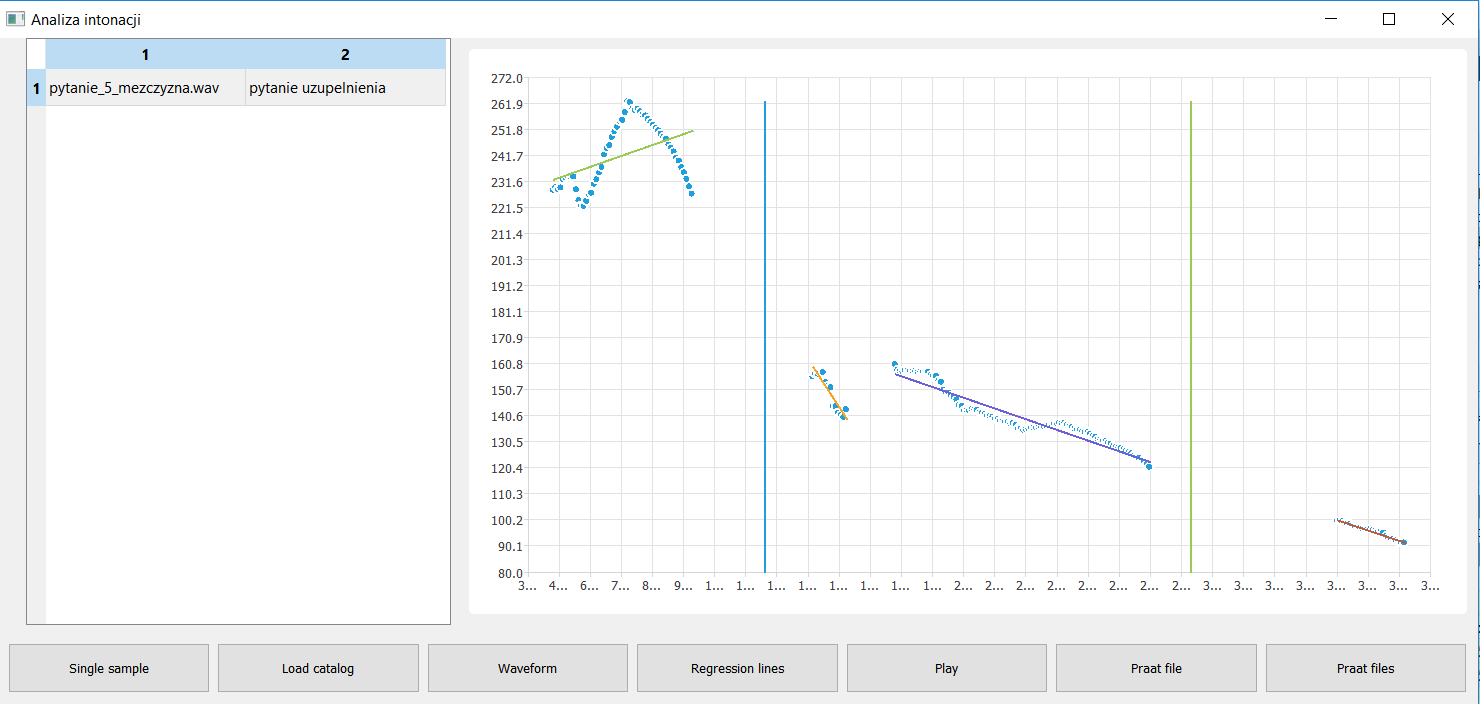
\includegraphics[scale=0.5]{gui.png}
\caption{Interfejs graficzny aplikacji}
\end{figure}
\FloatBarrier
\section{Wczytanie nagrania}
Pierwszym krokiem na drodze do rozpoznania rodzaju zdania, jest wczytanie calego nagrania przez program. Wykonuje sie to z wykorzystaniem mozliwosci oferowanych przez Qt. Framework oferuje do tego klase QAudioDecoder. 
Nagranie jest wczytywane w 100 milisekundowych fragmentach. Jako że częstotliwość próbkowania wynosi 44100Hz, na jeden fragment przypada 4410 wartości. Każda częśc jest odczytana jako obiekt klasy QAudioBuffer. Wektor typu QAudioBuffer zawiera cale wczytane nagranie.
\begin{lstlisting}[caption={Połączenie sygnałów niosących informacje o starcie lub zakończeniu wczytywania nagrania, ze slotami},label={lst:label},language=C++]
std::vector<QAudioBuffer>audioBuffers;
QAudioDecoder *audioDecoder;
\end{lstlisting}

\begin{lstlisting}
audioDecoder = new QAudioDecoder();
connect(audioDecoder, SIGNAL(bufferReady()), this, 
			SLOT(readBuffer()));
connect(audioDecoder,SIGNAL(finished()),this,
			SLOT(decodingFinished()));
audioDecoder->start();
\end{lstlisting}
Po wczytaniu kazdej z ramek emitowany jest sygnał. Łącząc sygnał ze slotem, możliwe jest przechwycenie aktualnie wczytanych wartości, zanim zostaną zastąpione wartościami kolejnej ramki.
Zostają one dodane do wektora ramek.
\begin{lstlisting}[caption={Funkcja przechwytująca wczytany fragment},label={lst:label},language=C++]
void MainWindow::readBuffer()
{
    audioBuffers.emplace_back(audioDecoder->read());
}
\end{lstlisting}
Gdy całe nagranie zostanie odczytane, QAudioDecoder emituje sygnał finished(). Po jego przechwyceniu, a więc otrzymaniu informacji o zakończeniu dekodowania, program umieszcza w jednym wektorze próbki ze wszystkich 100 milisekundowych buforów.

\begin{lstlisting}[caption={Funkcja dodająca do wektora wszystkie odczytane próbki},label={lst:label},language=C++]

void MainWindow::putValuesIntoVector()
{
    sampleRate = audioBuffers[0].format().sampleRate();
    frameSize = audioBuffers[0].format().sampleRate()/40;
    
    for (QAudioBuffer audioBuffer : audioBuffers)
    {
        const qint16 *data = audioBuffer.constData<qint16>();
        for(int j=0;j<audioBuffer.sampleCount();j++)
        {
              wholeBuffer.emplace_back(data[j]);
        }
        delete data;
    }
}
\end{lstlisting}
W powyższej funkcji, najpierw pobierana jest liczba próbek przypadających na jedną sekundę, oraz na 25 milisekundową ramkę. Następnie wartości kolejno z każdego obiektu typu QAudioBuffer, znajdującego się w wektorze audioBuffers, są dodawane do wektora wholeBuffer.

\section{Ekstrakcja tonu podstawowego}
W pierwotnym założeniu program, poza estymacją częstotliwości podstawowej miał również dokonywać ekstrakcji niskopoziomowych cech.
W toku implementacji zostały one jednak pominięte, z powodu posiadania małego wpływu na cel pracy. 
Pierwszym zagadnieniem, które było rozważone, jest długość fragmentów sygnału, na które powinien być podzielony.
Sygnały mowy nie są sygnalami stacjonarnymi, co oznacza, że ich częstotliwość istotnie zmienia się w czasie, znacznie obniżając dokładność obliczeń, opierających się na rezultatach transformaty Fouriera.
W przetwarzaniu mowy korzystne jest dzielenie sygnału na części, celem uzyskania fragmentów sygnału bliskich byciu stacjonarnymi.
Głośnia, odpowiedzialna za zmiany częstotliwości głosu, nie zamyka i nie otwiera się natychmiastowo, co oznacza, że w małych odstępach czasu wartości częstotliwości są do siebie zbliżone.
Odpowiednio dzieląc sygnał możliwe jest uzyskanie krótszych  quasi-stacjonarnych fragmentów. Proces ten nazywa się ramkowaniem.
\subsection{Ramkowanie oraz ekstracja wartości F0}
Sygnał najczęśniej dzielony jest na ramki o długości 20-50ms. W tym projekcie ustalona długość ramki wynosi 25ms. Oznacza to, że każda ramka składa się z 1102 wartości.
Pojawia się jednak problem związany z wartościami brzegowymi. Dzieląc sygnał na przystające do siebie, lecz nie zachodzące na siebie ramki istnieje duże ryzyko nie wykrycia pewnych cech, które mogą znajdować się pomiędzy dwoma kolejnymi ramkami. 
Taka sytuacja mogłaby wystąpić podczas analizy sygnału w celu wykrycia konturów częstotliwości podstawowej. Jeżeli relatywnie krótki kontur zaczynałby się w jednej ramce i kończył w drugiej, mógłby nie zostać wykryty.
Rozwiązaniem jest nakładanie ramek na siebie \textit{ang.overlapping}.Określona część każdej ramki, zawarta jest również w ramce kolejnej. Najczęściej jest to 20-50\% długości segmentu.
\begin{figure}[h]
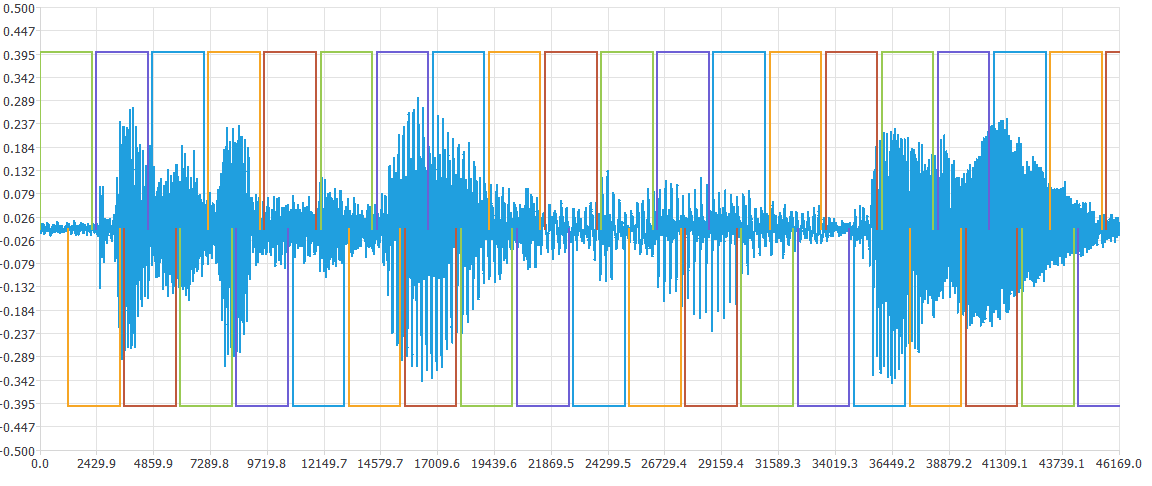
\includegraphics[scale=0.7]{overlapping.png}
\caption{Zobrazowany podział sygnału na ramki wraz zastosowaniem 30-procentowego zakładkowania. Opracowanie własne}
\end{figure}
\FloatBarrier
Do ekstrakcji cech niskopoziomowych 30 procentowe nakładanie się ramek jest wystarczające. Jednak algorytm YIN, wykorzystany w projekcie do estymacji F0, wymaga znacznie większego zachodzenia fragmentów na siebie. W tym przypadku 90\% danej ramki znajduje się również w ramce kolejnej.
Oznacza to, że ramki przesuwane są jedynie o 2,5ms. Spowodowane jest to faktem, że algorytm YIN opiera swoje działanie na funkcji autokorelacji.
Do ekstrakcji cech stworzona została klasa ExtractionHelper.
\FloatBarrier
\begin{figure}[h]
\centering
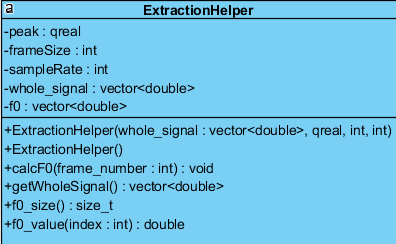
\includegraphics[scale=0.9]{featuresExtractor.png}
\caption{Klasa stworzona w celu ekstracji F0 oraz przechowywania tych wartości}
\end{figure}
\FloatBarrier
\newpage
\begin{lstlisting}[caption={Przedstawienie sposobu dokonywania podziału na ramki, wraz z zastosowaniem overlappingu},label={lst:label},language=C++]
void ExtractionHelper::calcF0(int numberOfFrames)
{
   int numberOfShifts=10;
   Yin m_yin(frameSize, sampleRate);
   int frameStartIndexAfterShifting = 0;
   int shift= frameSize/numberOfShifts;

   while(frameStartIndexAfterShifting < (whole_signal.size()))
   {
       double *shifted_frame =new double [frameSize];
       int index=0;
       frameStartIndexAfterShifting +=shift;
       for(int k=frameStartIndexAfterShifting;
		k<frameStartIndexAfterShifting+frameSize;k++)
       {
           if(k>=whole_signal.size())
              shifted_frame[index] = 0;
           else
              shifted_frame[index] = whole_signal.at(k);
           index++;
       }
       Yin::YinOutput f0_struct=m_yin.process(shifted_frame);
       if (f0_struct.f0 <F0_MAX && f0_struct.f0 >F0_MIN)
           f0.emplace_back(f0struct.f0);
       else
           f0.emplace_back(0);
       delete shifted_frame;
   }

}
\end{lstlisting}
W funkcji wykorzystywana jest klasa Yin, pochodząca z ogólnodostępnej implementacji algorytmu YIN. Konstruktor obiektu tej klasy jako argumenty przyjmuje długość pojedynczej ramki oraz częstotliwośc próbkowania.
W ciele funkcji calcF0 obiekt ten będzie wykorzystywany do estymacji konturów F0 dla pojedynczych ramek. 
Z racji zastosowania wysokiego overlappingu, proces dzielenia sygnału na fragmenty nie wygląda jak typowe ramkowanie. Okno sygnału przeznaczone do estymacji będzie przesuwane jedynie o 2,5ms.
W tym celu zadeklarowane zostały dwie zmienne, frameStartIndexAfterShifting przechowuje początkowy indeks obecnie przetwarzanej ramki, a zmienna shift przechowuje wartość pojedynczego przesunięcia.
Warunkiem kończącym działanie głównej pętli funkcji jest przekroczenie przez początkowy indeks ramki rozmiaru całego sygnału. Oznacza to, że końcowa ramka może być dowolnie mała.
W wewnętrznej pętli wartości rozpatrywanej ramki są przypisywane do dynamicznie zadeklarowanej tablicy. Jeżeli indeks tej pętli przekroczy rozmiar całego sygnału, reszta pól tablicy wypełniona jest zerami. Powodem tego jest wymaganie implementacji algorytmu YIN, aby wszystkie ramki miały jednakowy rozmiar.
Po zakończeniu estymacji wartości F0 dla danej ramki, wartość ta jest dodawana do wektoru jeżeli mieści się w zdefiniowanym zakresie. Musi być większa niż 60 i mniejsza niż 450. W przeciwnym razie do wektoru zostanie dodana wartość zerowa. Po obliczeniach zadeklarowana dla ramki pamięć zostaje zwolniona.
\section{Wykrywanie poszczególnych segmentów}
Wszystkie wyestymowane wartości częstotliwości podstawowej na tą chwilę przechowywane są w jednym wektorze. Aby umożliwić analizę przebiegu intonacji, konieczne jest wydzielenie poszczególnych segmentów. Segmentacji można dokonać analizując wartości pod kątem wartości odstających.
 Do tego celu zostały stworzone dwie klasy.
 \FloatBarrier
\begin{figure}[h]
\centering
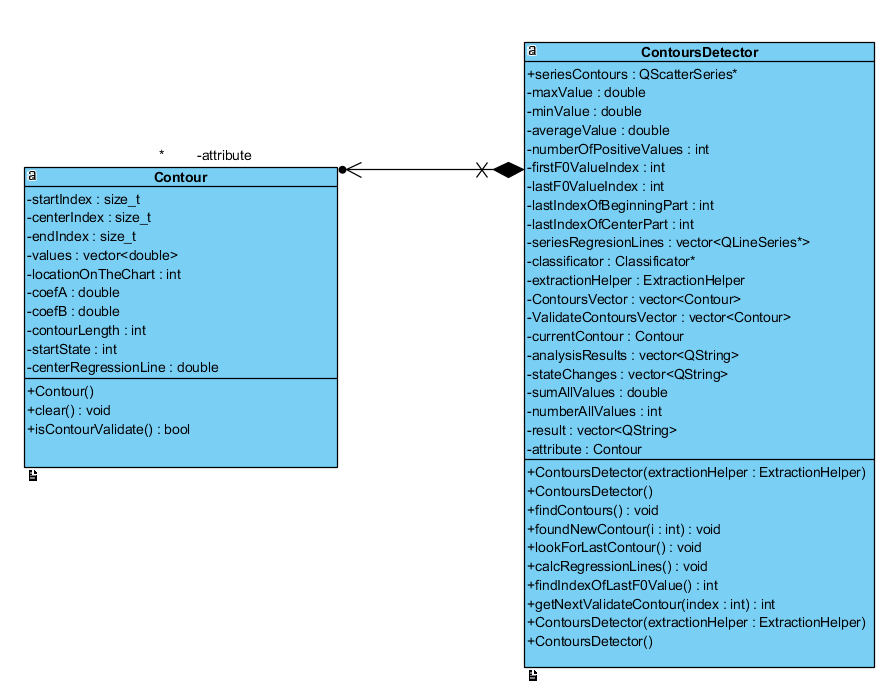
\includegraphics[scale=0.9]{contourDetector.png}
\caption{Klasy stworzone do wykrycia poszczególnych segmentów intonacyjnych, na podstawie wszystkich wartości F0}
\end{figure}
\FloatBarrier
Dla każdej ze zmiennych istnieją funkcje typu get i set, odpowiednio zwracające wartość zmiennej oraz przypisujące dana wartość. Zostały one pominięte w celu zwiększenia czytelności diagramów.
Główna funkcjonalność zawarta jest w funkcji findContours() w klasie ContoursDetector. Wykryte kontury będą umieszczane jako obiekty typu Contour, w wektorze contoursVector. W wektorze tym będą również umieszczane fragmenty z wartościami zerowymi, dla których nie wykryto występowania intonacji. Będą one pomijane w dalszej analizie, dodawane są w celu ułatwienia przejrzystego wyświetlania konturów na wykresie, w miejscu w którym rzeczywiście się znajdują.

\newpage
\begin{lstlisting}[caption={Początkowa faza funkcji wykrywającej segmenty},label={lst:label},language=C++]
#define TRANSITION 15

void ContoursDetector::findContours()
{
    currentContour.setStart(1);
    lastValueIndex = findIndexOfLastF0Value();
    for(size_t i=1;i<extractionHelper.f0_size();i++)
    {
        double value =extractionHelper.f0_value(i);
        double previousValue = extractionHelper.f0_value(i-1); 
        seriesContours->append(i,value);
        if (value > maxValue) maxValue = value;
        if (value < minValue && value > F0_MIN) minValue = value;
        if(std::abs(value - previousValue) > TRANSITION)
        {
            currentContour.setEnd(i-1);
  	    currentContour.setCenter();    
            foundNewContour();
            currentContour.setStart(i);
            currentContour.addValue(value);
        }
        else
        {
            currentContour.addValue(value);
        }
    }
    
\end{lstlisting}
Początkowy indeks pierwszego segmentu jest ustawiony jako 1. Główna pętla przebiega po wszystkich wyestymowanych wartościach tonu podstawowego. Oprócz poszukiwania segmentów, wartości są również sprawdzane pod kątem wykrycia wartości maksymalnej i minimalnej. Funkcja uznaje wykrywanie danegosegmentu za zakończone, gdy aktualnie rozpatrywana wartość rózni się od poprzedniej o 15 jednostek. Metodą obserwacji ustalono taki przeskok za wystarczający do stwierdzenia, że dana wartość należy już do nowego segmentu. Poprzedzający indeks jest uznawany za koniec danego segmentu. Aktualny licznik pętli zostaje przekazany do funkcji foundNewContour. Z uwagi na obszerność tej funkcji, będzie ona omawiana fragmentami.
\subsection{Analiza wstępna wykrytego fragmentu}
\begin{lstlisting}[caption={Funkcja zajmująca się analizą wstępną wykrytego segmentu},label={lst:label},language=C++]
void ContoursDetector::foundNewContour()
{
    if (!currentContour.isContourValidate())
    {
        currentContour.clear();
        return;
    }
    ContoursVector.push_back(currentContour);
    currentContour.clear();
}    
                
\end{lstlisting}
Najpierw segment jest poddawany walidacji. Sprawdzane jest, czy nie występują w nim wartości zerowe oraz czy jego długość jest większa niż 1. Przyjęta implementacja segmentacji traktuje wartości zerowe jako przerwy między fragmentami i nie powinny one być dodawane do wektoru przechowującego wykryte segmenty. Do określania czy dany obiekt jest przerwą między segmentami, wystarczy sprawdzić jego pierwszą wartość.
Metodą obserwacji zauważono, że te składające się tylko z jednej wartości, często są błędami estymacji, lub powstają w wyniku róznego rodzaju zanieczyszczeń w nagraniu. Mogą zaburzać wyniki późniejszej klasyfikacji, dlatego są pomijane.
\begin{lstlisting}[caption={Funkcja dokonująca walidacji segmentu},label={lst:label},language=C++]
    bool isContourValidate()
    {
        if (values.size()<2) return false;
        if (values.at(0) == 0)  return false;
        return true;
    }
\end{lstlisting}

Następnie kontur zostaje dodany do wektoru,  zmienna currentContour zostaje wyczyszczona w celu poszukiwania kolejnego konturu. Na tym funkcja foundNewContour kończy swoje działanie.

\begin{lstlisting}[caption={Dalsza część głównej funkcji findContours},label={lst:label},language=C++]

    double averageWithoutCurrentContour;
    for(int i = 0;i<ContoursVector.size();)
    {
        averageWithoutCurrentContour = sumAllValues - 
        ContoursVector.at(i).getCenterOfRegressionLine();
        averageWithoutCurrentContour /= (ContoursVector.size()-1);
        if((ContoursVector.at(i).getCenterValue() 
        	> (averageWithoutCurrentContour*1.5))
                && (ContoursVector.at(i).getContourLength()<10))
        {
            ContoursVector.erase(ContoursVector.begin()+i);
        }
        else
        {
            i++;
        }
    }
    calcRegressionLines();
 }
\end{lstlisting}
W czasie implementacji wykrywania konturów oraz przy późniejszej analizie, zauważano występowanie krótkich, wyraźnie odstających fragmentów. Pojawiały się w miejscach, w których nie było logicznego uzasadnienia ich występowania. Miały wyraźny wpływ na zaburzenia procesu wykrywania rodzaju zdania.
Podjęto decyzję o usuwaniu ze zbioru takie segmenty, których wartości są bardzo wyraźnie większe od średniej oraz jednocześnie są bardzo krótkie. Pierwotnie zostało to zaimplemetowane w celach testowych, lecz okazało się, że zabieg ten znacząco poprawia stopień poprawnego rozpoznawania.
 \FloatBarrier
\begin{figure}[h]
\centering
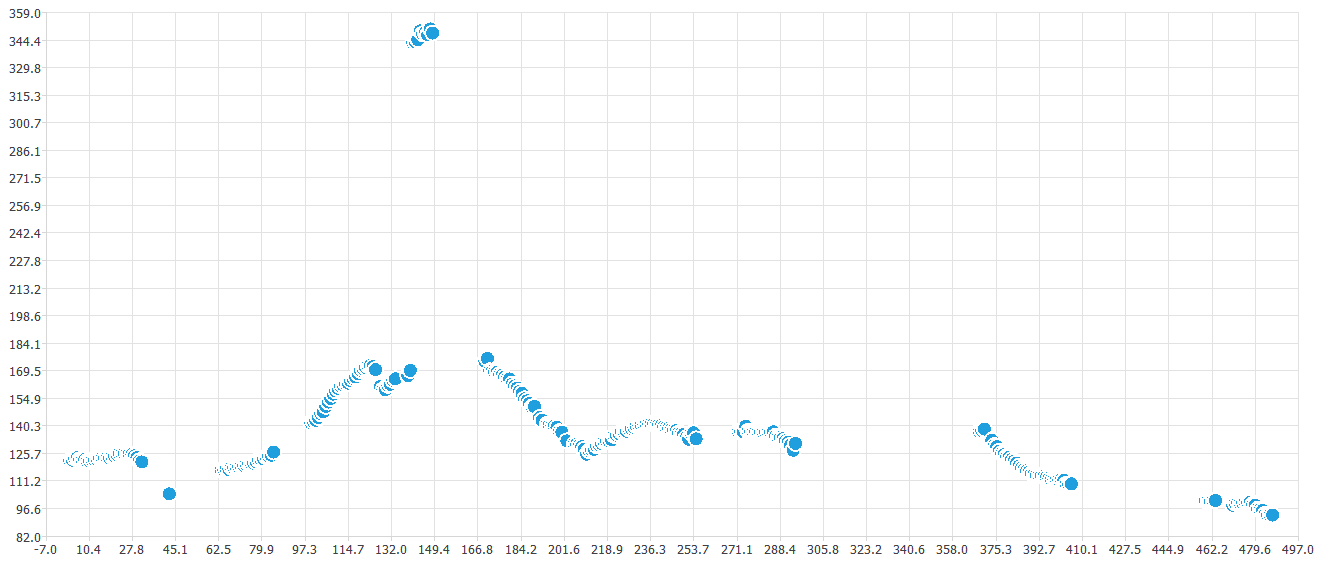
\includegraphics[scale=1.0]{usuniety_kontur.png}
\caption{Przykład usuniętego segmentu.}
\end{figure}
\FloatBarrier
Na rysunku 14 przedstawiony został przykład usuniętego segmentu. Jest to segment, którego wartości oscylują około 345 jednostek. Jest to liczba ponad dwukrotnie większa od innych, do tego fragment ten jest bardzo krótki.
Słuchając nagrania, nie sposób było uzasadnić jego występowanie w tym miejscu, dlatego został uznany za błąd estymacji i usunięty ze zbioru. 



\subsection{Współczynniki regresji liniowej}
Dla każdego wykrytego segmentu obliczane są współczynniki regresji liniowej. W tym celu została zaimplementowana metoda najmniejszych kwadratów.
Kod tej funkcji nie został umieszczony w pracy, z uwagi na jego obszerność oraz fakt, ze jest to implementacja  znanego algorytmu. Wewnątrz funkcji, każdemu fragmentowi zostają przypisane wartości obliczonych współczynników A i B oraz obiekt typu QLineSeries. Obiekt ten, bazując na obliczonych współczynnikach, słuzy do zobrazowania na wykresie przebiegu linii regresji dla danego segmentu.
 \FloatBarrier
\begin{figure}[h]
\centering
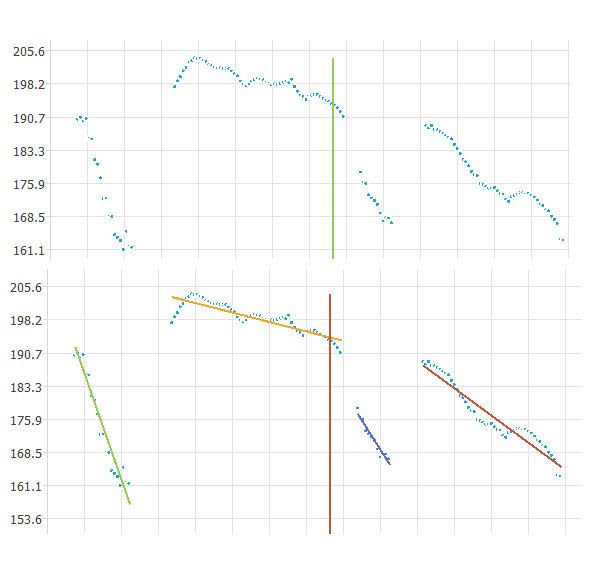
\includegraphics[scale=0.7]{regresja.png}
\caption{Fragment przebiegu intonacji przed i po nałożeniu linii regresji}
\end{figure}
\FloatBarrier
\section{Wczytywanie wartości  uzyskanych za pomocą programu PRAAT}
PRAAT jest programem służącym do analizy, przetwarzania oraz syntezy mowy. Został stworzony dla środowiska naukowego i jest powszechnie używany w badaniach poświęconych mowie. W zakresie jego możliwości znajduje się również ekstrakcja częstotliwości podstawowej. Wartości te następnie moga być zapisane do pliku tekstowego w następującej formie:

\begin{tabular}{c r @{} l}
Time\_s &
\multicolumn{2}{c}{F0\_Hz}\\ \hline
0.023469 & --undefined-- \\
0.033469 & --undefined-- \\
0.033469 & 327.395121 \\
0.023469 &  --undefined-- \\
0.033469 &  --undefined-- \\
0.043469 &  --undefined-- \\
0.053469 &  --undefined-- \\
0.063469 &  --undefined-- \\
0.073469 &  327.395121 \\
0.083469 &  322.101395 \\
0.093469 &  314.760925 \\
0.103469 &  311.135612 \\
\end{tabular}



Wartości estymowane są co 10 milisekund. Brak wykrytej wartości w danym momencie, oznaczany jest przez PRAATa jako ''--undefined--''.
\begin{lstlisting}[caption={Funkcja wczytująca do programu wartości F0 z pliku tekstowego},label={lst:label},language=C++]
void MainWindow::processPraatFile(QString filepath)
{
    praatFilesNumber++;
    QFile file(filepath);
    if(!file.open(QIODevice::ReadOnly)) 
        QMessageBox::information(0, "error", file.errorString());

    std::vector<double> f0;
    while(!in.atEnd()) {
        QString line = in.readLine();
        std::string stringLine = line.toStdString().substr(11,line.size());
         line = QString::fromStdString(stringLine);
        double value;
        if(line.at(0) == '-')
            value = 0.0;
        else
            value = line.toDouble();
        f0.emplaceback(value);
      }

    file.close();
    ExtractionHelper exHelper;
    exHelper.setF0(f0);
    ContoursDetector contoursDetector(exHelper);
    contoursDetector.findContours();
    contoursDetector.classification();
  }
\end{lstlisting}
Zadaniem przedstawionej funkcji jest wczytanie do programu wartości częstotliwości podstawowej uzyskanych za pomocą PRAATa, przechowywanych w pliku tekstowym. Funkcja najpierw sprawdza czy dany plik istnieje i czy da się go otworzyć. Następnie wczytywane są kolejno wszystkie linie tego pliku. Z wczytanej linii uzyskiwany jest podzbiór znaków, jako, że wartości F0 zaczynają się w 11 kolumnie każdej z linii. Jak zostało już wspomniane, pauzy w przebiegu intonacji oznaczone są jako ''--undefined--'', więc pierwszy znak tego podzbioru porównywany jest ze znakiem ''-''. Jeżeli porównanie zwróci wartość prawdziwą, do wektoru przechowującego wczytane wartości, wczytane zostanie zero. W przeciwnym razie wczytany podzbiór jest konwertowany do wartości typu zmiennoprzecinkowego o podwójnej precyzji, a nastepnie dodany do wektoru. Gdy wszystkie wartości zostaną wczytane, plik jest zamykany, a wektor wczytanych wartości poddawany jest segmentacji oraz analizie.
\chapter{Analiza wykrytych segmentów}
Po zakończeniu implementacji segmentacji konturów oraz obliczania współczynników regresji liniowej, kolejnym etapem pracy była analiza wykrytych segmentów. Celem tej analizy było wykrycie wszelkiego rodzaju cech, które powtarzałyby się w zdaniach tego samego typu, a więc mogły by być użyteczne w procesie klasyfikacji zdań. 
Analizowane były takie własciwosci przebiegu intonacji jak:
\begin{itemize}
\item{gwałtowne wzrosty/spadki częstotliwosci podstawowej w całym przebiegu }
\item{ogólna tendencja zmian konturu}
\item{ilosc oraz długosć poszczególnych segmentów}
\end{itemize}

Szybko została zauważona istotna własciwosć konturów. Dla niektórych zdań wartosci F0 były bardzo wysokie na początku nagrania, dla innych z kolei gwałtowny wzrost nastąpywał na samym końcu.

\section{Pytania rozstrzygnięcia}
W pierwszej kolejności nagrania były analizowane pod kątem rozpoznania ich jako pytania rozstrzygnięcia. Ten rodzaj wypowiedzi cechuje się silną antykadencją zlokalizowaną w końcowej częsci zdania.
Jest to najbardziej charakterystyczny rodzaj zdania, dlatego program zaczyna klasyfikacje od niego.
 \FloatBarrier
\begin{figure}[h]
\centering
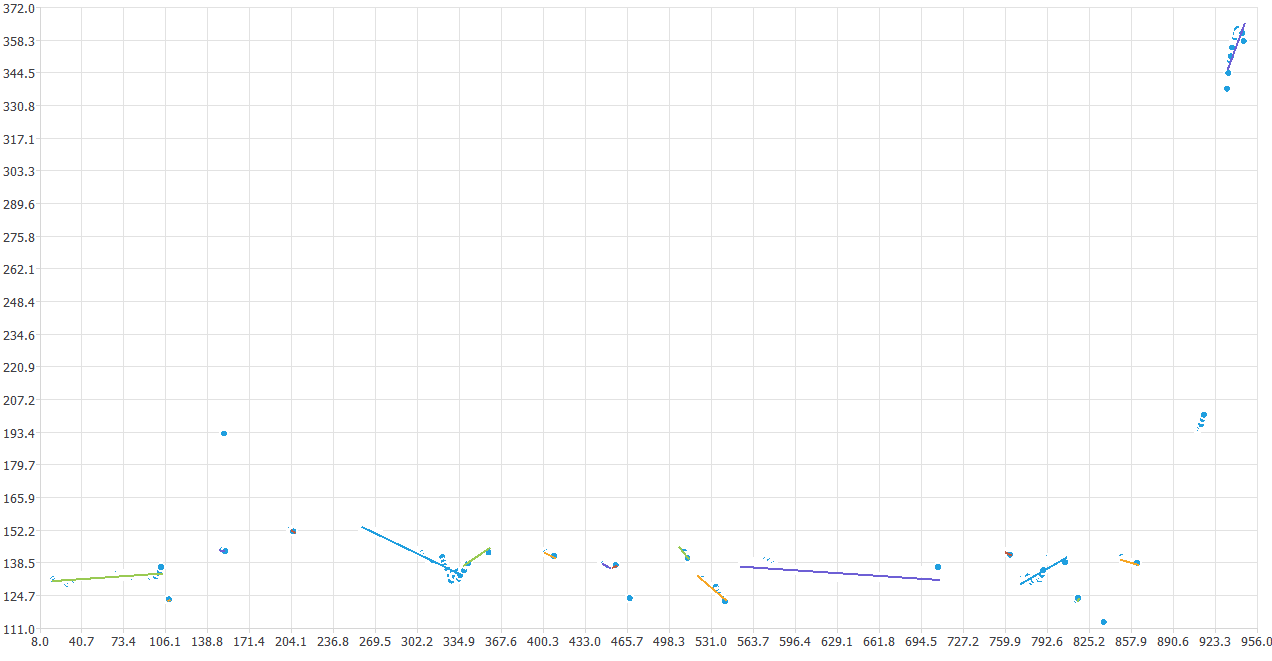
\includegraphics[scale=0.6]{pytanie_rozstrzygniecia.png}
\caption{Pytanie rozstrzygnięcia zadane przez mężczyznę}
\end{figure}
\FloatBarrier
Pytanie przedstawione na rysunku 10 brzmi 'Faktycznie jest gdzies w Tobie taka pasja?'. Jest ono wypowiedziane przez mężczyznę. Nie ma w tej wypowiedzi żadnego słowa, które wyraźnie wskazywałoby na to, że jest to pytanie, a nie stwierdzenie. Jednak, dzięki nadaniu wypowiedzi odpowiedniej intonacji, możliwe jest rozpoznanie jej jako pytanie - zarówno przez program, jak i przez człowieka. W przedstawionym przykładzie, wzrost intonacji na końcu nagrania jest bardzo wyraźny, znacznie przekracza zakres typowych częstotliwosci F0 uzyskiwanych w głosie męskim. Dla pytań rozstrzygnięcia dosć charakterystyczne jest to, że ogólna tendencja intonacji wcale nie musi być rosnąca, zazwyczaj ten wzrost następuje gwałtowanie, dla jednego lub kilku końcowych segmentów. W danym przykładzie, przed wystąpieniem akcentu intonacyjnego w ostatnim słowie, intonacja utrzymywała się na stałym poziomie. Nie może jednak być to uznane za regułę, co udowodni kolejny przykład.
 \FloatBarrier
\begin{figure}[h]
\centering
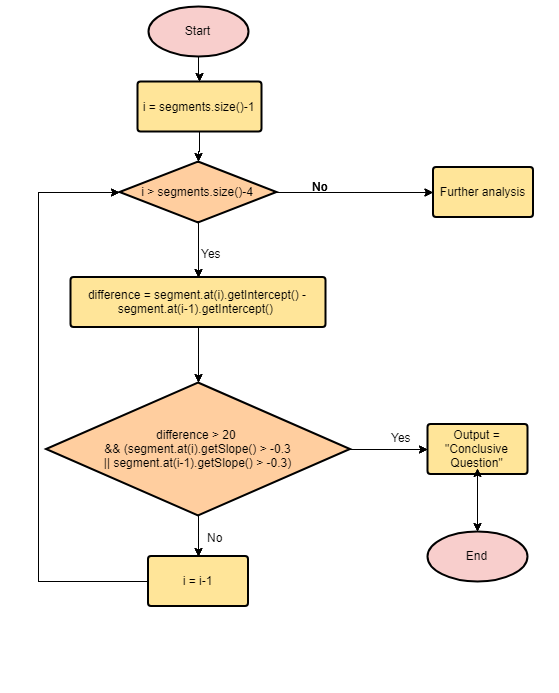
\includegraphics[scale=1.0]{conclusive.png}
\caption{Schemat rozpoznawania pytań rozstrzygnięcia}
\end{figure}
\FloatBarrier
Na rysunku 11 przedstawiony został algorytm rozpoznawania pytań rozstrzygnięcia, w przebiegu których nastąpił gwałtowny wzrost wartości F0 w ostatniej fazie wypowiedzi. Pod uwagę brane są trzy ostatnie kontury. Porównywane jest położenie  (\textit{ang.intercept}), oraz sprawdzane jest nachylenie (\textit{ang.slope}) przypisanej do sąsiadujących segmentów linii regresji. Jeżeli róznica w położeniu segmentów jest znacząca, a do tego przynajmniej jeden z nich nie jest gwałtownie opadający, wypowiedź zostaje rozpoznana jako pytanie rozstrzygnięcia.
 \FloatBarrier
\begin{figure}[h]
\centering
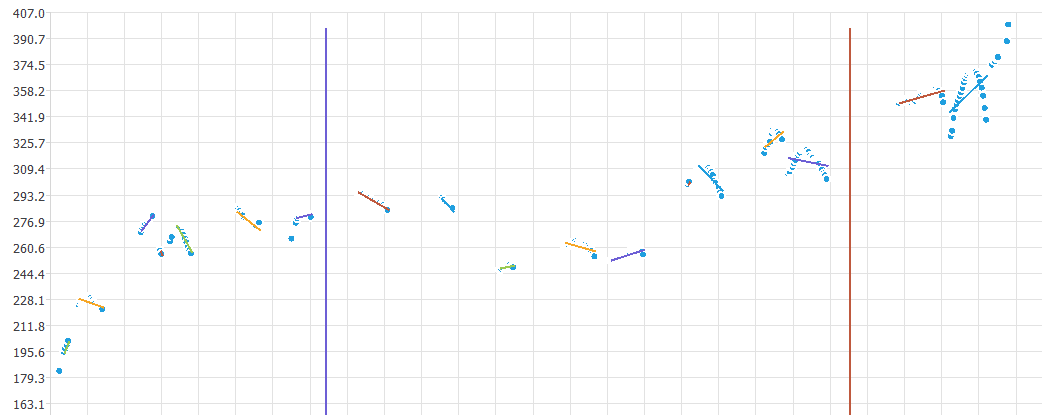
\includegraphics[scale=0.6]{pytanie_rozstrzygniecia_2_emocje.png}
\caption{Pytanie rozstrzygnięcia z nacechowaniem emocjonalnym}, wypowiedziane przez mężczyznę
\end{figure}
\FloatBarrier
Pytanie, którego intonacja została przedstawiona na rysunku 12, brzmi ''Może o to, że jest to rażąco niesprawiedliwe?'' Zostało wypowiedziane przez mężczyzne. Nosi ono również znamiona pytania retorycznego.  W tej wypowiedzi nie ma gwałtowanego wzrostu intonacji na samym końcu nagrania, zamiast tego intonacja zauważalnie rosnie w trakcie całej wypowiedzi. Mimo, że jest to nagranie głosu męskiego, wyestymowane wartosci F0 znacznie wykraczają poza zakres typowy dla mężczyzn. Spowodowane jest to dużym zabarwieniem emocjonalnym wypowiedzi.
 \FloatBarrier
\begin{figure}[h]
\centering
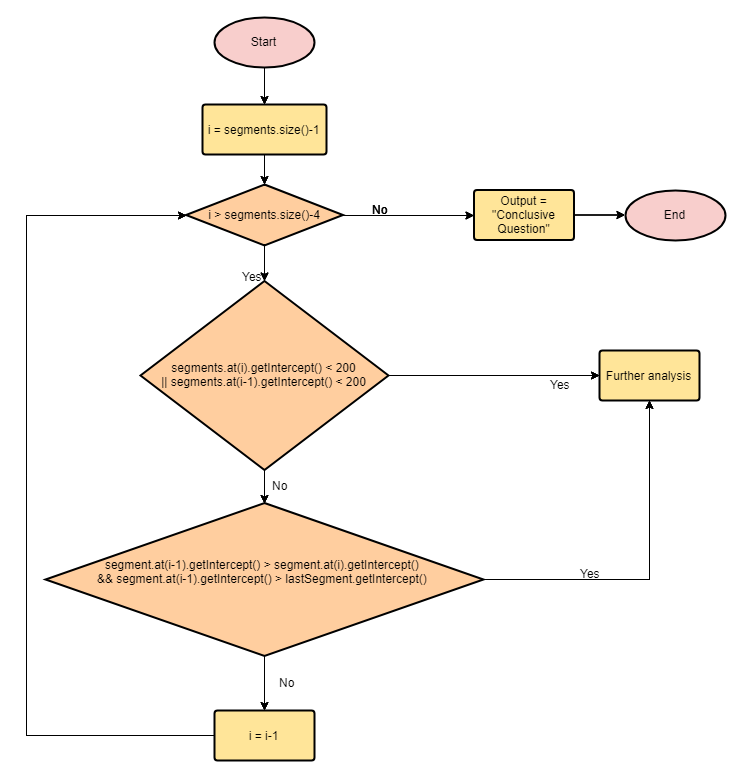
\includegraphics[scale=0.9]{conclusive2.png}
\caption{Schemat rozpoznawania pytań rozstrzygnięcia z tendencją rosnącą}
\end{figure}
\FloatBarrier
Na rysunku 13 przedstawiony został algorytm rozpoznawania pytań rozstrzygnięcia, w przebiegu których nie wystąpił gwałtowny wzrost wartości F0 w ostatniej fazie wypowiedzi lecz ogólna tendencja intonacji była rosnąca.
Ponownie pod uwagę brane są ostatnie trzy kontury. Jako ,że zaobserwowane zostało występowanie wysokich wartości F0 w przypadku tego rodzaju pytań, jako pierwsze sprawdzane jest położenie segmentów. Jeżeli uzyskane wartość dla któregoś z sąsiadujących segmentów jest mniejsza od 200, wypowiedź na pewno nie jest pytaniem rozstrzygnięcia. Jeżeli warunek jest spełniony, program porównuje połozenie badanych segmentów. Jeżeli segment znajdujący się bliżej początku jest położony wyżej od porównywanego z nim segmentu oraz dodatkowo leży wyżej również od ostatniego segmentu, intonacja nie może być postrzegana jako rosnąca, a zatem wypowiedź nie jest pytaniem rozstrzygnięcia. Tym sposobem zostało rozpoznane pytanie przedstawione na rysunku 12.
 \FloatBarrier
\begin{figure}[h]
\centering
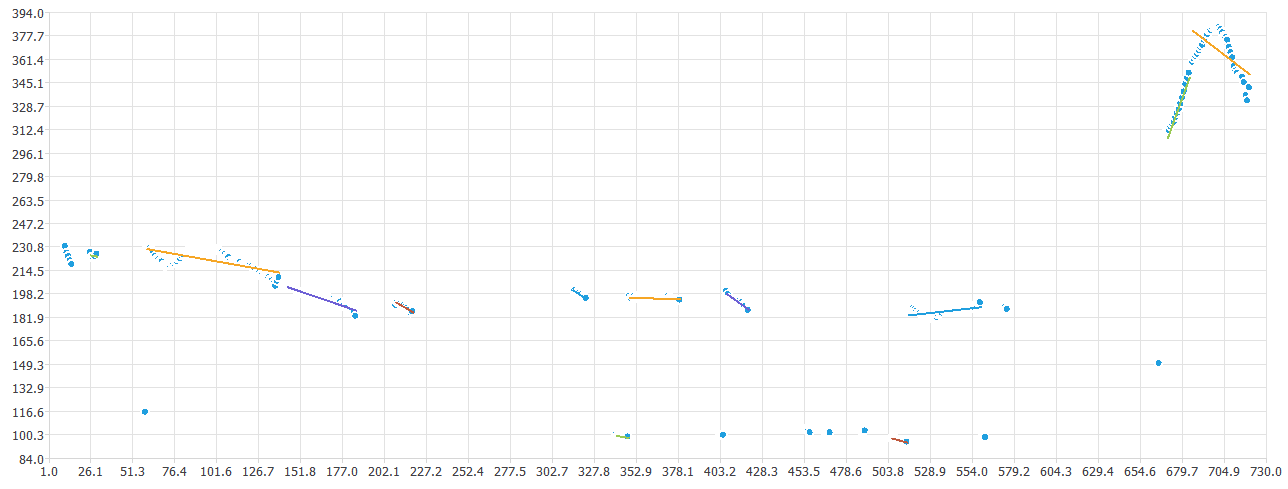
\includegraphics[scale=0.65]{pytanie_rozstrzygniecia_3_kobieta.png}
\caption{Pytanie rozstrzygnięcia zadane przez kobietę}
\end{figure}
\FloatBarrier
Ostatnie z przedstawionych pytań rozstrzygnięcia zostało wypowiedziane przez kobietę. Brzmi ono ''A czy Tobie marzy się kariera zagraniczna?''.  Przebieg intonacji jest zbliżony do przykładu przedstawionego na rysunku 10, tutaj również tendencja intonacji nie jest rosnąca, lecz następuje silny skok intonacji na końcu wypowiedzi.
\section{Pytania dopełnienia}
Intonacja nadawana pytaniom dopełnienia całkowicie różni się od opisanej dla pytań rozstrzygnięcia. W tym przypadku zaobserwowany został brak jakiekolwiek wzrostu intonacji w końcowej częsci wypowiedzi, oraz cały przebieg intonacji jest najczęsciej opadający. Tresc tych wypowiedzi jawnie wskazuje, że jest to pytanie, ponieważ na ich początku zawarty jest zaimek pytajny. Przykłady takich zaimków to ''kto, dlaczego, który, czemu, jak, co''. Charakterystyczny dla tego rodzaju pytań jest wysoko zaintonowany początek wypowiedzi,  po którym następuje znaczny spadek estymowanych wartosci.
 \FloatBarrier
\begin{figure}[h]
\centering
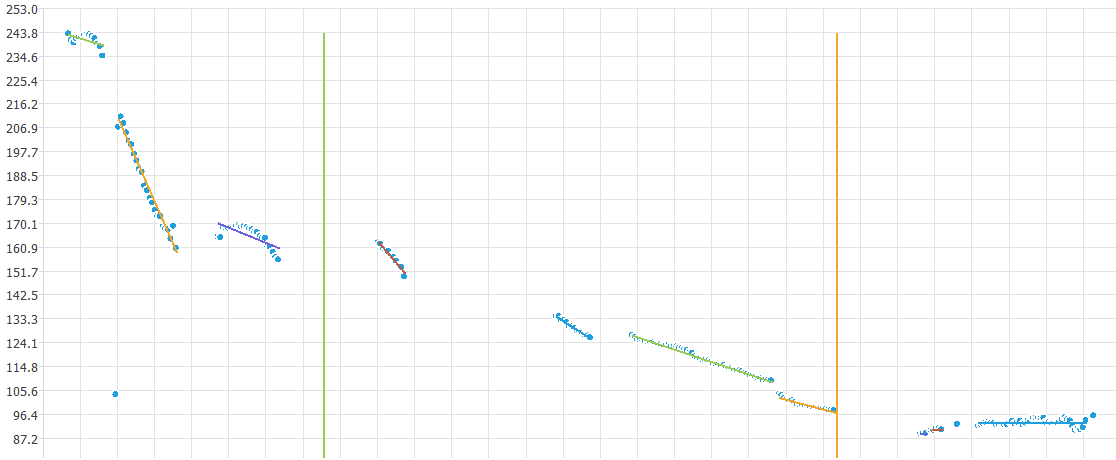
\includegraphics[scale=0.55]{pytanie_uzupelnienia_marynarz.png}
\caption{Pytanie dopełnienia zadane przez mężczyznę}
\end{figure}
\FloatBarrier
Pytanie, którego intonacja została przedstawiona na rysunku 13, zostało wypowiedziane przez mężczyznę. Jego tresć to ''Jak zostać marynarzem?''. Na pierwszy rzut oka zauważalny jest pierwszy segment, którego wartosci górują nad resztą wykresu. W wypowiedzianym pytaniu, duży nacisk intonacyjny został nałożony na zaimek pytajny, po czym nastąpił znaczny spadek wartosci F0. Cała intonacja jest wyraźnie opadająca. Jako, że zaimek występujący w tym zdaniu składa sie jedynie z trzech liter, odpowiadający mu segment również jest krótki. Istotne jest również to, że wartosci kolejnych segmentów są mniejsze aż o 80-140Hz w porównaniu do segmentu położonego najwyżej.

 \FloatBarrier
\begin{figure}[h]
\centering
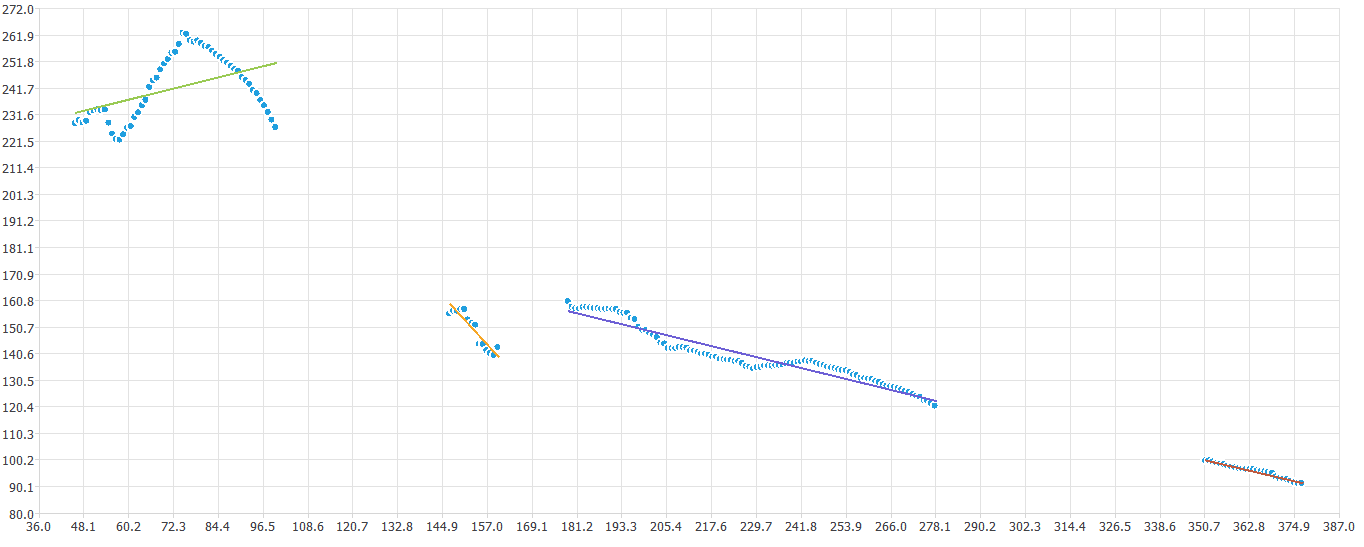
\includegraphics[scale=0.55]{pytanie_dopelnienia_2.png}
\caption{Pytanie dopełnienia zadane przez mężczyznę}
\end{figure}
\FloatBarrier
Treść pytania przedstawionego na rysunku 16 brzmi ''Czego Cię to nauczyło?''. Również zostało wypowiedziane przez mężczyznę. W tym pytaniu także najwyżej położony segment jest znacznie większy od pozostałych. Nacisk położony na zaimek pytajny jest wyraźnie widoczny.
 \FloatBarrier
\begin{figure}[h]
\centering
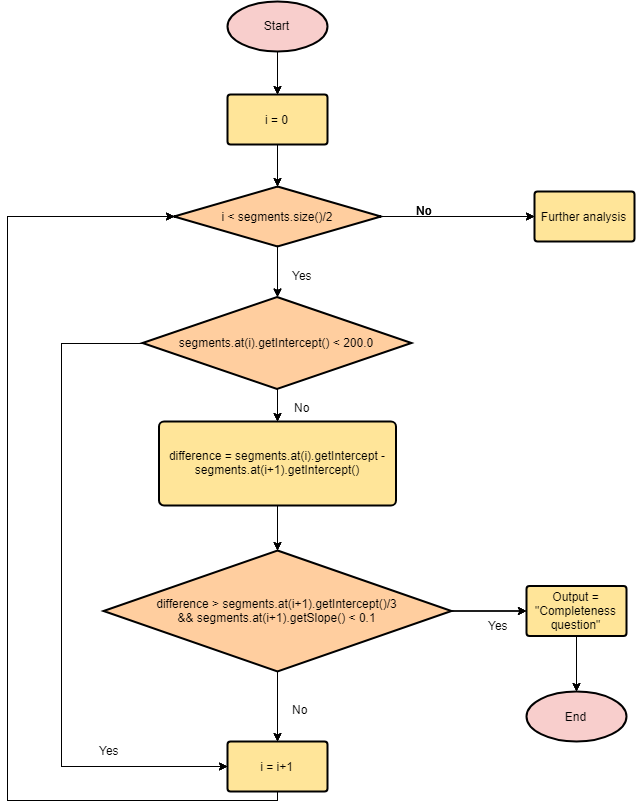
\includegraphics[scale=0.85]{completeness.png}
\caption{Schemat rozpoznawania pytań dopełnienia}
\end{figure}
\FloatBarrier
Rysunek 17 przedstawia schemat rozpoznawania pytań dopełnienia. Ten rodzaj wypowiedzi charakteryzuje się wysokimi wartościami intonacji na początku wypowiedzi, zazwyczaj towarzyszy im późniejszy znaczny spadek wartości.
Pod uwagę brana jest pierwsza połowa zbioru segmentów. Najpierw program sprawdza czy dany segment jest położony wystarczająco wysoko. W przeciwnym razie segment ten zostaje ominięty. Następnie obliczona zostaje różnica w położeniu między sąsiadującymi segmentami.
Aby zdanie zostało sklasyfikowane jako pytanie dopełnienia, różnica między nimi musi być większa niż wartość położenia niżej znajdującego się segmentu, podzielona na trzy. Zauważono, że z racji dużych różnic między wartościami F0 uzyskiwanymi dla kobiet i mężczyzn, takie porównanie jest wydajniejsze niż porównywanie ze stałą wartością. Dodatkowymi warunkiem klasyfikacji jest brak rosnącej tendencji niżej położonego segmentu.

\section{Zdania rozkazujące}
Dla pytań dopełnienia charakterystyczna jest obecnosć krótkich segmentów o wysokich wartosciach zlokalizowanych na początku przebiegu intonacji. W przypadku pytań rozstrzygnięcia, taki charakterystyczny segment obecny był na końcu wypowiedzi. W zdaniach nakazujących komus wykonanie jakiej czynnosci, kładziony jest silny akcent na czasownik. W skutek tego, najczęsciej segmenty o największych wartosciach F0 zlokalizowane są w centralnej częsci przebiegu intonacji, lub zaczynają się w początkowej częsci, kończąc w srodkowej. Z racji nałożonego na nie akcentu, dosć często są najdłuższymi segmentami w danej wypowiedzi. W tym przypadku funkcja gramatyczna intonacji przeplata się z funkcją podkreślającą znaczenie danego słowa. Zaprezentowane zostanie 5 różnych grup cech wskazujących na ten rodzaj zdania.
Pierwszym krokiem jest znalezienie najwyżej położonego segmentu w pierwszej połowie zbioru.
 \FloatBarrier
\begin{figure}[h]
\centering
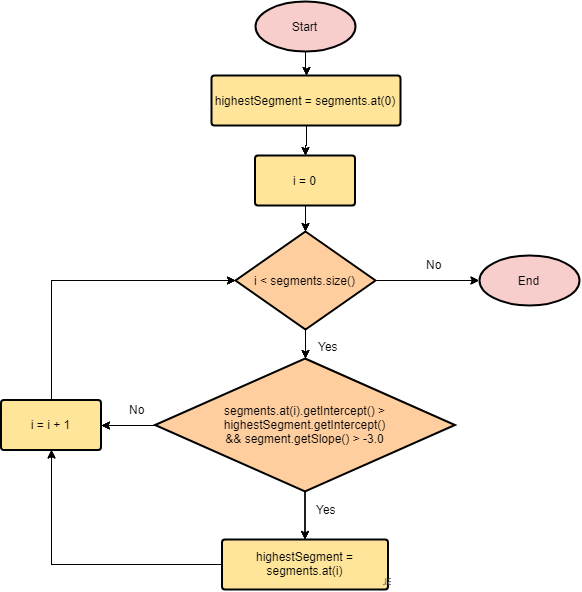
\includegraphics[scale=0.9]{HighestDetection.png}
\caption{Schemat wykrywania najwyżej położonego segmentu}
\end{figure}
\FloatBarrier
Aby dany segment został uznany za najwyżej zlokalizowany, oprócz położenia musi spełniać jeszcze jeden warunek. Nie może być to segment silnie, wręcz pionowo, opadający.
 \FloatBarrier
\begin{figure}[h]
\centering
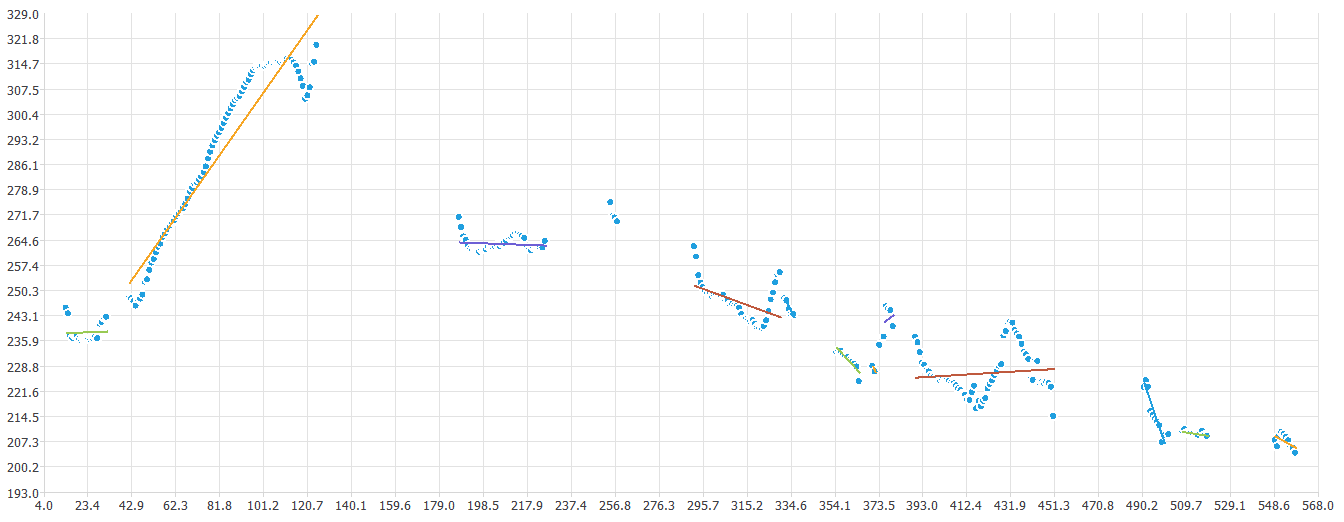
\includegraphics[scale=0.6]{rozkaz_1_kobieta.png}
\caption{Zdanie rozkazujące wypowiedziane przez kobietę}
\end{figure}
\FloatBarrier

Zdanie przedstawione na rysunku 19 zostało wypowiedziane przez kobietę, a jego treść brzmi ''Wyłącz w końcu ten telewizor''. Najwyżej położony segment odpowiada czasownikowi oraz gwałtownie rośnie będąc jednocześnie najdłuższym segmentem w zbiorze. Są to cechy wskazujące na zdanie rozkazujące. 
Zostało wykryte przez fragment algorytmu, który został przedstawiony na rysunku 20.
 \FloatBarrier
\begin{figure}[h]
\centering
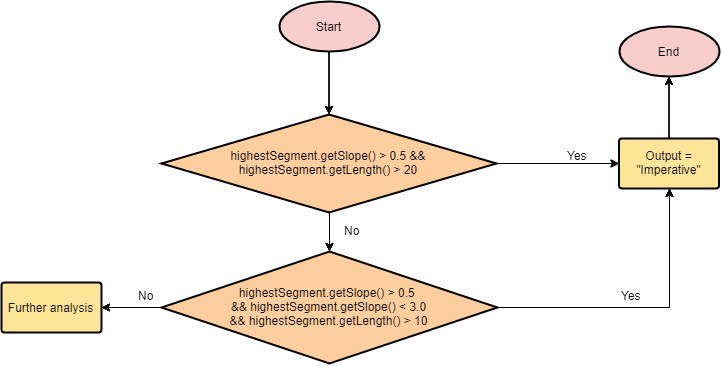
\includegraphics[scale=0.9]{Imperative1.png}
\caption{Schemat wykrywania zdania rozkazującego zawierającego pierwszą grupę cech}
\end{figure}
\FloatBarrier
W tym fragmencie algorytmu, program podejmuje próbę rozpoznania zdania jako rozkazującego, bazując na nachyleniu oraz długości najwyżej położonego segmentu.
Jeżeli długość danego segmentu jest większa niż 20 jednostek i jednocześnie segment jest silnie rosnący, właściwości te wskazują na zdanie rozkazujące. Jeżeli jednak jest krótszy, wciąz może wskazywać na zdanie rozkazujące, jeżeli nie jest ostro rosnący. Ta cecha jest odrzucana przez program, ponieważ zaobserwowano jej związek ze zdaniami twierdzącymi. Jeśli zdanie nie spełnia żadnego z tych warunków, jest poddawane dalszej analizie.

 \FloatBarrier
\begin{figure}[h]
\centering
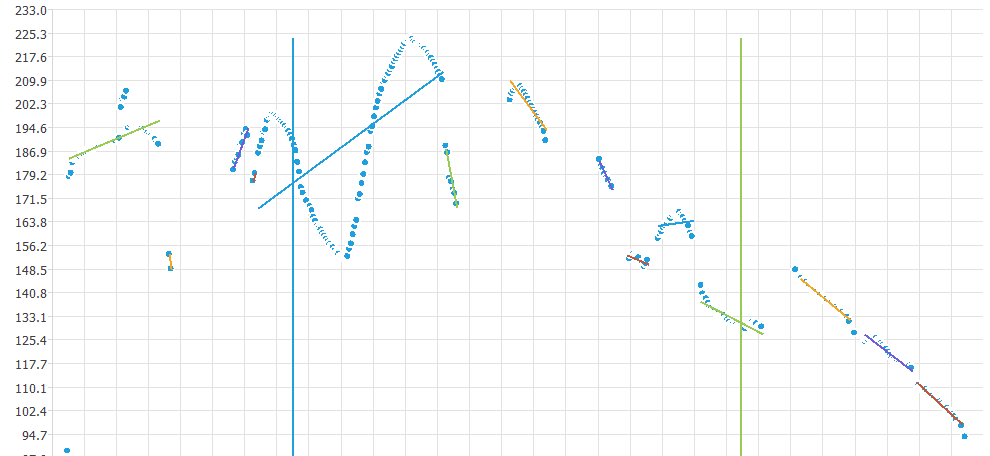
\includegraphics[scale=0.6]{rozkaz_dom.png}
\caption{Zdanie rozkazujące wypowiedziane przez mężczyznę}
\end{figure}
\FloatBarrier
Zdanie przedstawione na rysunku 21 zostało wypowiedziane przez mężczyznę, a jego treść brzmi ''Nie próbujcie tego w domu''. Wyraźny akcent w tej wypowiedzi jest położony na drugie słowo, sylaby w czasowniku są wręcz przeciagnięte, a więc wykorzystany został również iloczas. Na skutek tego omawiany segment poza największymi wartościami, odznacza się również długością. Kolejną zauważalną cechą jest jego gwaltowny wzrost, zakończony krótkim spadkiem. 

 \FloatBarrier
\begin{figure}[h]
\centering
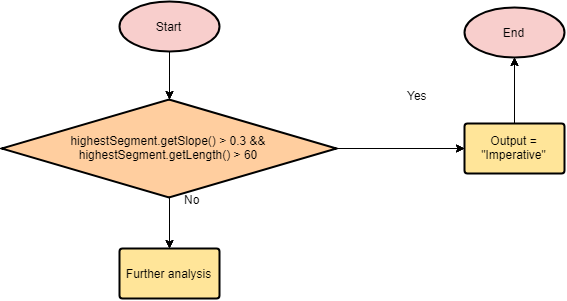
\includegraphics[scale=0.9]{Imperative2.png}
\caption{Schemat wykrywania zdania rozkazującego zawierającego drugą grupę cech}
\end{figure}
\FloatBarrier
Zdanie może zostać rozpoznane jako rozkazujące, również gdy jego nachylenie jest słabo rosnące, ale za to jest to znacząco długi segment. Długość segmentu odzwierciedla nacisk położony na czasownik. Przykład przedstawiony na rysunku 21 został zidentykowany w ten sposób. Badany segment odpowiada naciskowi nałożonemu na słowo ''próbujcie''.
 \FloatBarrier
\begin{figure}[h]
\centering
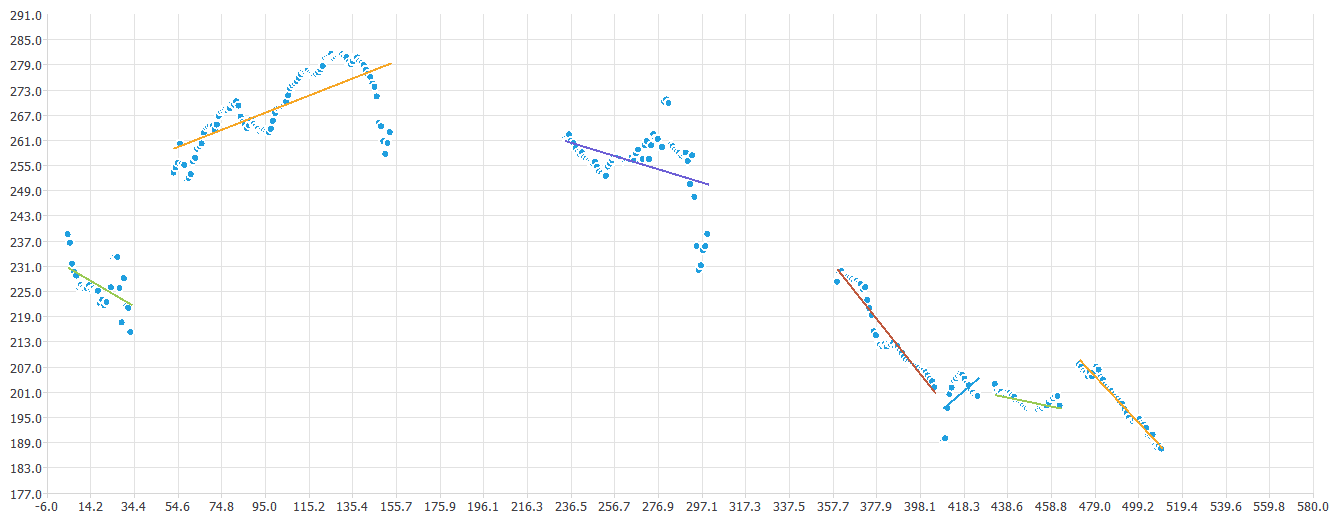
\includegraphics[scale=0.6]{rozkaz_3.png}
\caption{Zdanie rozkazujące wypowiedziane przez kobietę}
\end{figure}
\FloatBarrier
Zdanie przedstawione na rysunku 23 zostało wypowiedziane przez kobietę, a jego treść brzmi ''Wynieś śmieci jak wrócisz''. Akcent intonacyjny ponownie nałożony jest na czasownik w trybie rozkazującym, lecz tym razem jedynie na jego drugą oraz trzecią sylabę. Po pierwszej zauważalna jest krótka pauza.
W tym przypadku najistotniejszy segment jest opadający, co pokazuje, że nie zawsze jest rosnący jak w poprzednich przykładach i nie może być ta właściwość traktowana jako powszechna cecha.
 \FloatBarrier
\begin{figure}[h]
\centering
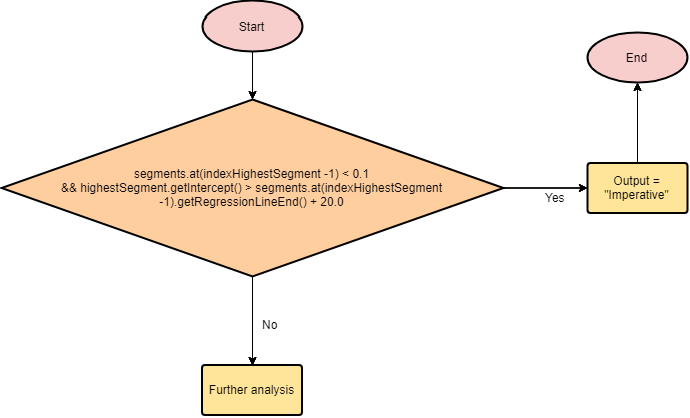
\includegraphics[scale=0.85]{Imperative3.png}
\caption{Schemat wykrywania zdania rozkazującego zawierającego trzecią grupę cech}
\end{figure}
\FloatBarrier
Rysunek 24 przedstawia warunki, po których spełnieniu zdanie z rysunku 23 zostało sklasyfikowane jako zdanie rozkazujące. Ta gałąź algorytmu sprawdza czy segment poprzedzający najwyżej zlokalizowany segment jest opadający. Jeżeli warunek jest spełniony, sprawdzana jest różnica między położeniem najwyższego segmentu z położeniem końca segmentu poprzedzającego. Duży przeskok w takim przypadku wskazuje na zdanie rozkazujące. Jeżeli dane warunki nie zostaną spełnione, program kontynuuje analizę zdania.
 \FloatBarrier
\begin{figure}[h]
\centering
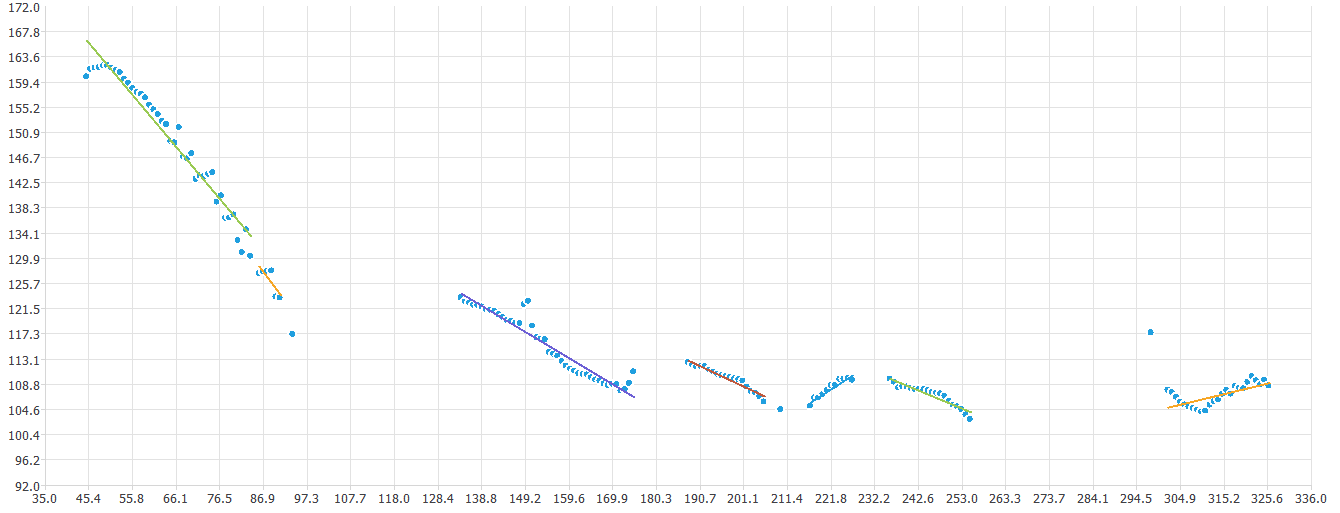
\includegraphics[scale=0.6]{rozkaz_4.png}
\caption{Zdanie rozkazujące wypowiedziane przez mężczyznę}
\end{figure}
\FloatBarrier
Intonacja tego zdania przypomina przebieg intonacji występujący przy pytaniach dopełnienia. Jednak w tym przypadku różnica między najwyżej położonym segmentem, a następnym segmentem nie była wystarczająco duża, aby rozpoznać je jako pytanie. Kluczowe dla rozpoznania tego zdania jako zdania rozkazującego jest nachylenie obu segmentów. Jeżeli oba są dłuższe niż 10 jednostek oraz są to segmenty opadające, zdanie zostaje rozpoznane jako zdanie rozkazujące.

Warunek, po którego spełnienie te zdanie zostało sklasyfikowane jako rozkazujące, przedstawiony jest na rysunku 26.
 \FloatBarrier
\begin{figure}[h]
\centering
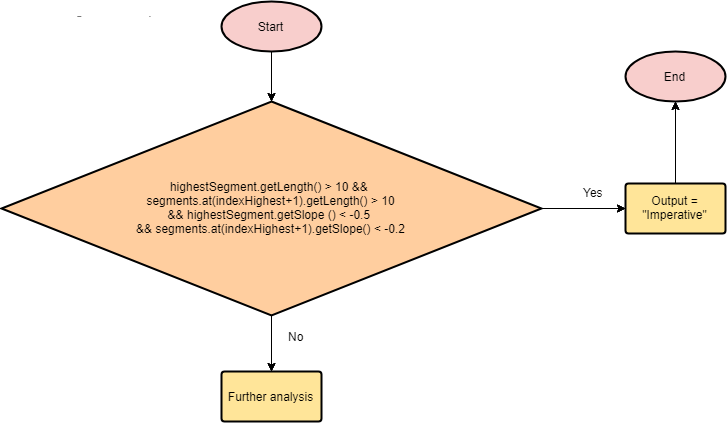
\includegraphics[scale=0.9]{Imperative4.png}
\caption{Schemat wykrywania zdania rozkazującego zawierającego czwartą grupę cech}
\end{figure}
\FloatBarrier
 \FloatBarrier
\begin{figure}[h]
\centering
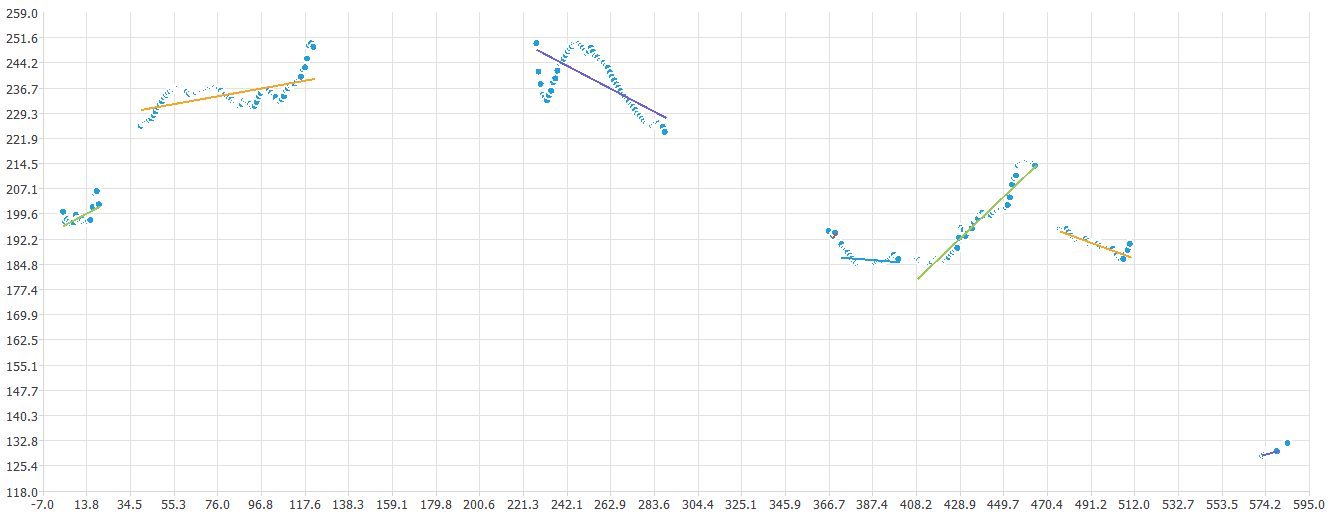
\includegraphics[scale=0.6]{rozkaz_5_kobieta.png}
\caption{Zdanie rozkazujące wypowiedziane przez kobietę}
\end{figure}
\FloatBarrier
Treść rozkazu przedstawionego na rysunku 27 brzmi ''Zanieś zakupy do domu''. Zdanie zostało wypowiedziane przez kobietę. Charakterystyczna jest obecność dość długiej przerwy zaraz po najbardziej znaczącym segmencie.

 \FloatBarrier
\begin{figure}[h]
\centering
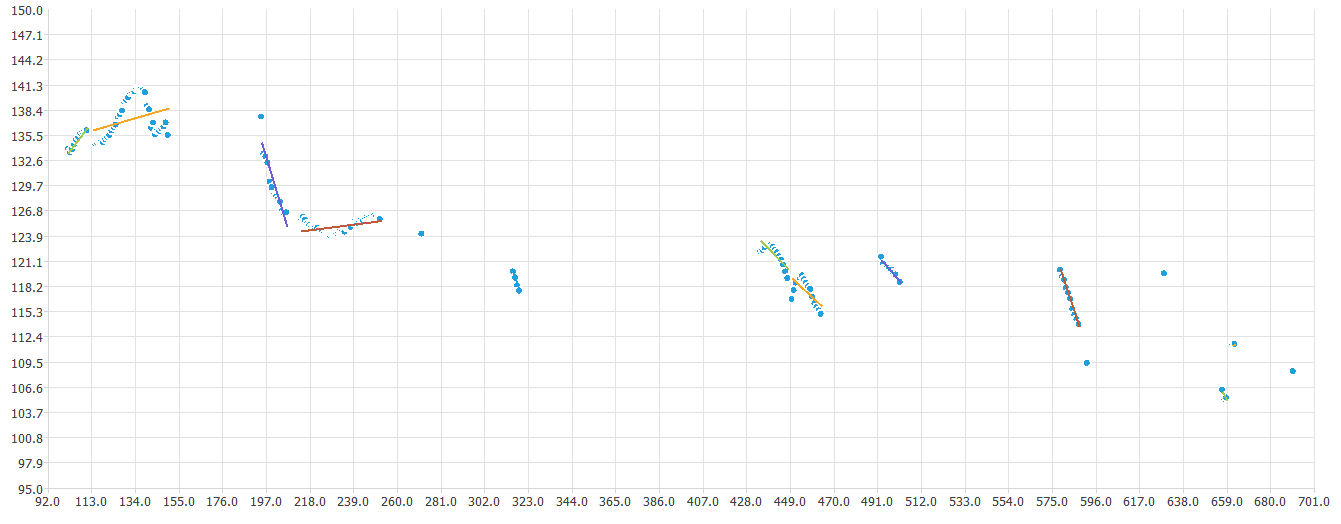
\includegraphics[scale=0.6]{rozkaz_6.png}
\caption{Zdanie rozkazujące wypowiedziane przez mężczynę}
\end{figure}
\FloatBarrier
Zdanie przedstawione na rysunku 28 brzmi ''Skończ najpierw sprzątać swój pokój''. Zauważalne są te same cechy co w zdaniu poprzednim. Bazując na tych obserwacjach opracowany został ostatni warunek rozpoznania zdania rozkazującego, przedstawiony na rysunku 29. Zdanie zostaje uznane za rozkazujące, jeśli najwyżej położony segment jest wystarczająco długi, nie opada stromo, oraz przerwa między nim, a kolejnym segmentem jest większa niż długość najwyższego segmentu.
 \FloatBarrier
\begin{figure}[h]
\centering
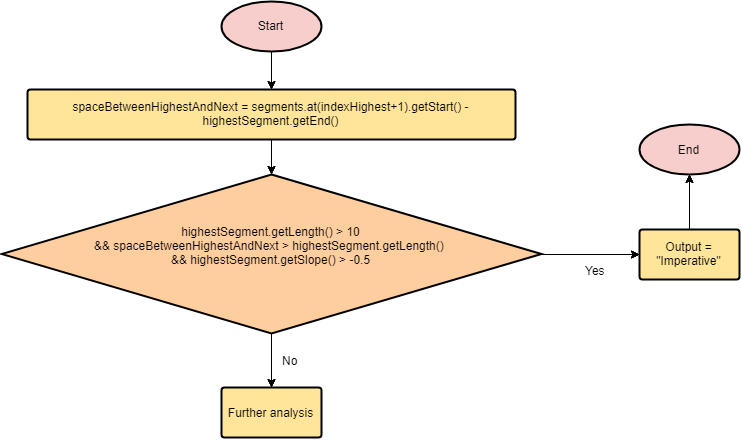
\includegraphics[scale=0.9]{Imperative5.png}
\caption{Schemat wykrywania zdania rozkazującego zawierającego piątą grupę cech}
\end{figure}
\FloatBarrier

\subsection{Zdania twierdzące}
Podczas obserwacji intonacji zdań twierdzących zauważono stałą lub delikatnie opadającą tendencję. Nie występują w nich nagłe wzrosty lub spadki wartości F0 na początku wypowiedzi. Brak w nich również gwałtwnych wzrostów lub wysokich wartości na końcu zdania, tak charakterystycznych dla pytań rozstrzygnięcia.
W przypadku opadającego przebiegu intonacji, spadek wartosci ma łagodny charakter. Wpływ na to ma fakt, że zdania te są zazwyczaj wypowiadane bez zabarwienia emocjonalnego, ich główną funkcją jest przekazanie informacji.W porównaniu do wcześniej analizowanych rodzajów zdań, w przypadku zdań twierdzących intonacja ma najmniejszy wpływ na postrzeganie tych zdań przez człowieka.



 \FloatBarrier
\begin{figure}[h]
\centering
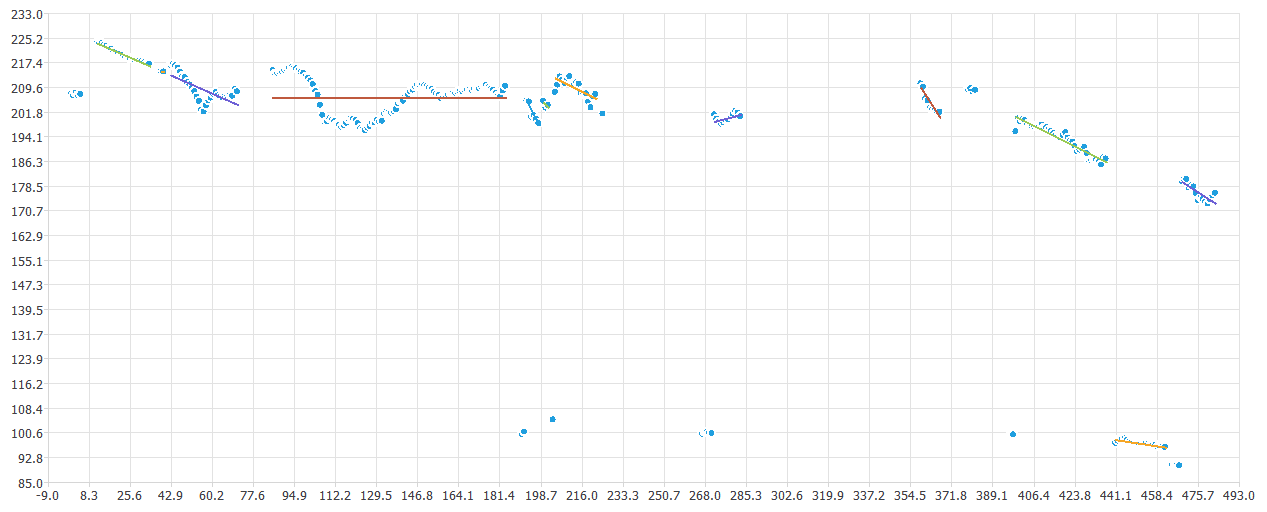
\includegraphics[scale=0.6]{twierdzenie_1_kobieta.png}
\caption{Zdanie twierdzące wypowiedziane przez kobietę}
\end{figure}
\FloatBarrier
Zdanie przedstawione na rysunku 30 przedstawia zdanie twierdzące, którego intonacja przedstawia stałą tendencję. Zostało wypowiedziane przez kobietę, a jego treść brzmi ''Zawsze byli bardzo wspierający''. Średnie wartości kolejnych segmentów są bardzo do siebie zbliżone. Najwyżej zlokalizowany segment jest delikatnie opadający, dodatkowo brak większej przerwy między nim, a następnym segmentem.


 \FloatBarrier
\begin{figure}[]
\centering
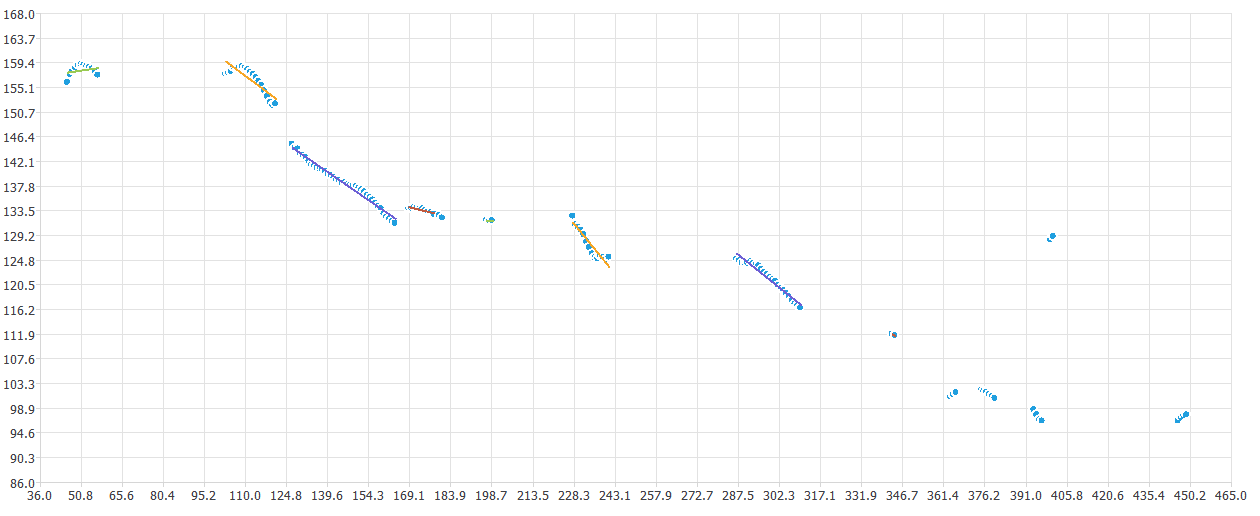
\includegraphics[scale=0.6]{twierdzenie_2_mezczyzna.png}
\caption{Zdanie twierdzące wypowiedziane przez mężczyznę}
\end{figure}
\FloatBarrier

Zdanie przedstawione na rysunku 31 zostało wypowiedziane przez mężczyznę, a jego tresć brzmi ''W zeszłym roku ten las wycięto''. Największe wartosci intonacji zostały zauważone dla słów ''W zeszłym'' lecz spadek wartosci dla segmentów odpowiadających kolejnym słowom jest dosć łagodny. Dopiero ostatnie słowo ma wyraźnie niższą intonację. Główną cechą zdań twierdzących pozwalających rozróżnić ten rodzaj wypowiedzi od pytań dopełnienia jest niewielka różnica między wartosciami najwyższego segmentu, a otoczającymi segmentami. W przypadku pytań dopełnienia ta różnica potrafiła wynosić nawet 100Hz i znacznie wykraczać poza typowy zakres częstotliwosci. Ten przebieg intonacji jest wręcz idealnym przykładem zdania twierdzacego, średnie wartosci każdego segmentu są mniejszego od segmentu poprzedniego, przy tym nie wystepuja gwałtownego spadki między nimi oraz wszystkie segmenty są opadające.

\begin{figure}[h]
\centering
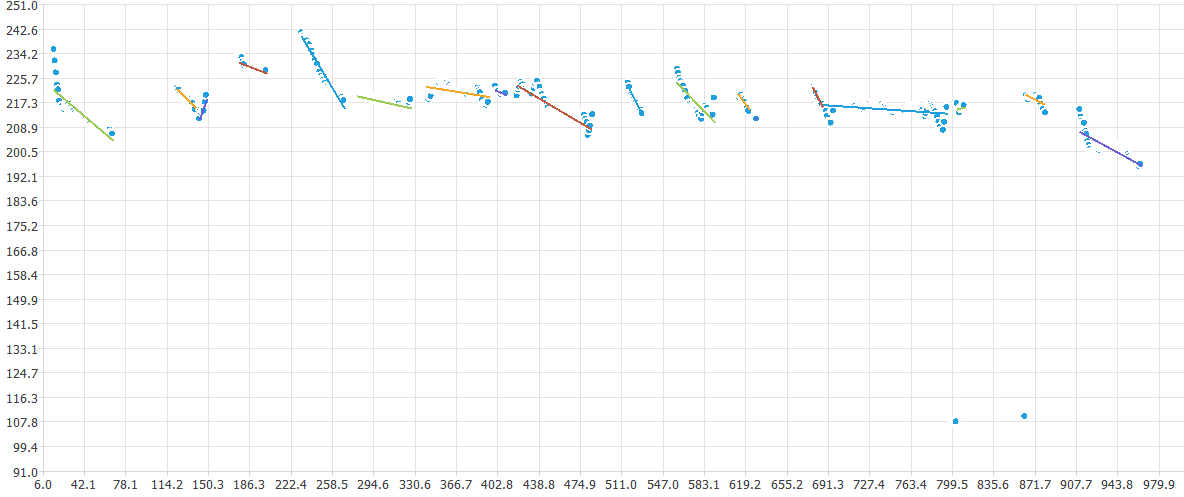
\includegraphics[scale=0.7]{twierdzenie_3_kobieta.png}
\caption{Zdanie twierdzące wypowiedziane przez kobietę}
\end{figure}
\FloatBarrier
Przykład przedstawiony na rysunku 32, przedstawia przebieg intonacji zdania twierdzącego, wypowiedzianego przez kobietę, którego tresć brzmi ''Więc to też naraża ich na niebezpieczeństwo''. W tym przykładzie przebieg intonacji również ma wyraźnie stałą tendencję. Nie sposób tutaj mówić o znaczącej różnicy między średnią wartością segmentu zlokalizowanego najwyżej, a otaczającymi go segmentami. Stała tendencja przebiegu intonacji jest jedną z cech wyraźnie wskazujących, że dana wypowiedź jest zdaniem twierdzącym.

 
\section{Porównanie wyników otrzymanych z wykorzystaniem YIN i Praata}
Jednym z założeń pracy było porównanie wyników uzyskanych przez proponowaną metodę rozpoznawania, dla konturów wykrytych za pomocą dwóch różnych metod ekstrakcji F0. W tym celu dla każdego z nagrań znadujących sie w bazie uczącej przygotowano plik z wartościami F0 uzyskanymi przez PRAAT-a. Wartości te następnie są wczytywane do programu będącego efektem tej pracy, dzielone na segmenty oraz analizowane.
Tendencje przebiegów intonacji uzyskane za pomocą PRAAT-a sa takie same jak te uzyskane z użyciem algorytmu YIN. Różnice moga być obserwowane jedynie w długościach poszczególnych segmentów, na co wpływ ma zastosowany sposób dzielenia intonacji na segmenty.


Poprawność klasyfikacji dla intonacji uzyskanej za pomocą PRAAT-a jest nieznacznie gorsza od tej uzyskanej dla segmentów opartych na algorytmie YIN. Większa ilość błędnych rozpoznań została zaobserwowana dla zdań rozkazujących. Warunki rozpoznania tych zdań są oparte w istotnym stopniu na wartościach nachylenia segmentów oraz odległościach między nimi. Wartości progowe były ustalone metodą obserwacyjną. Kontury uzyskane za pomocą PRAAT-a zachowują podobną tendencję, lecz inna metoda ekstrakcji powoduje, że w poszczególnych przypadkach parametry te istotnie się różnią.

\subsection{Pytania rozstrzygnięcia oraz dopełnienia}
Metoda rozpoznawania pytań sprawdza się równie dobrze, bez względu na źródło pochodzenia wartości F0.

\begin{figure}[h]
\centering
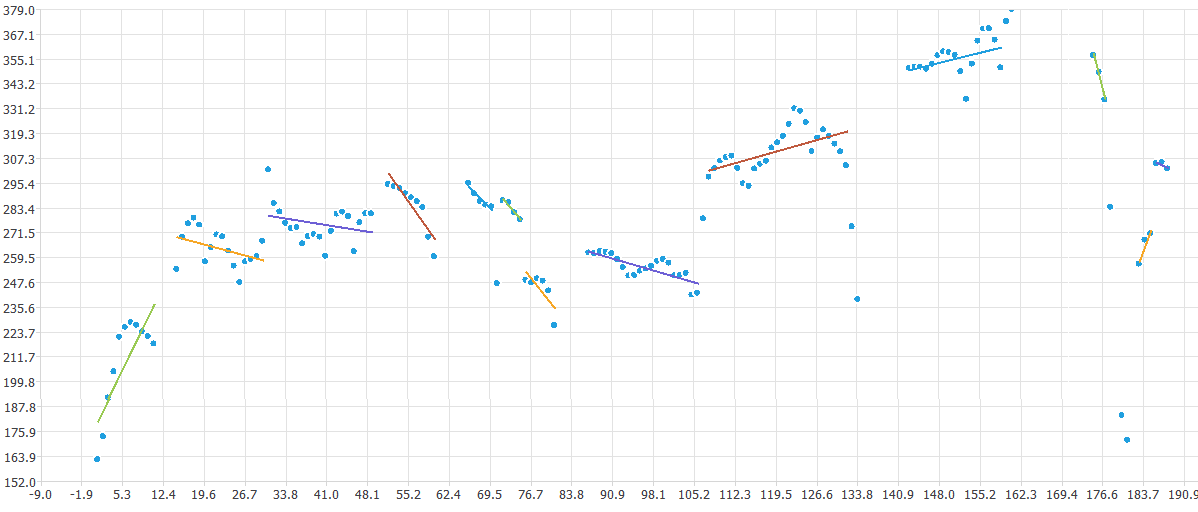
\includegraphics[scale=0.7]{pytanie_rozstrzygniecia_2_emocje_praat.png}
\caption{Intonacja pytania przedstawionego na rysunku ... lecz uzyskana za pomocą PRAAT-a}
\end{figure}
\FloatBarrier
Rosnąca tendencja intonacji została wykryta również gdy uzyskane segmenty oparte były na wartościach F0 pochodzących z PRAAT-a.

\begin{figure}[h]
\centering
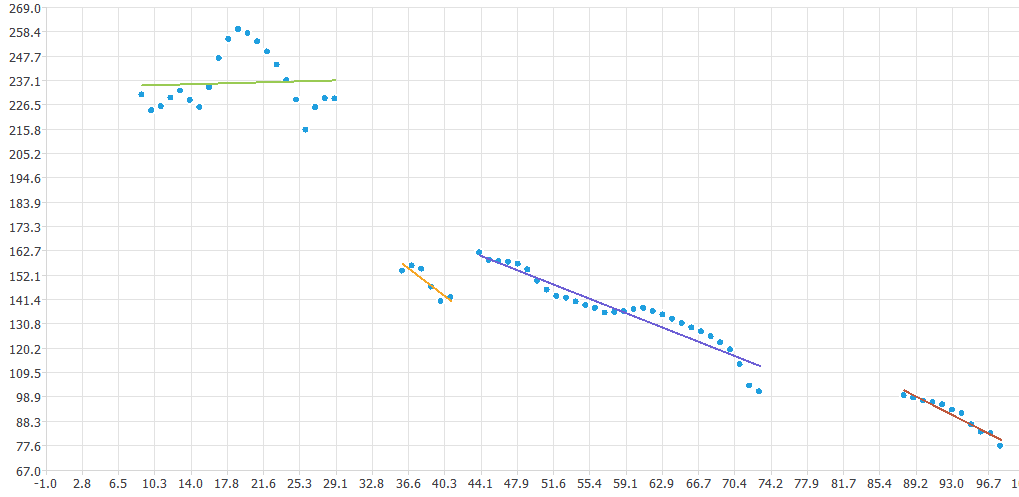
\includegraphics[scale=0.7]{pytanie_dopelnienia_praat_2.png}
\caption{Intonacja pytania przedstawionego na rysunku ... lecz uzyskana za pomocą PRAAT-a}
\end{figure}
\FloatBarrier

W przypadku pytań dopełnienia, gwałtowne spadki między najwyżej zlokalizowanym segmentem oraz następnym segmentem są wykrywane bez względu na sposób pochodzenia wartości F0.

\subsection{Zdania rozkazujące oraz zdania twierdzące}
\begin{figure}[h]
\centering
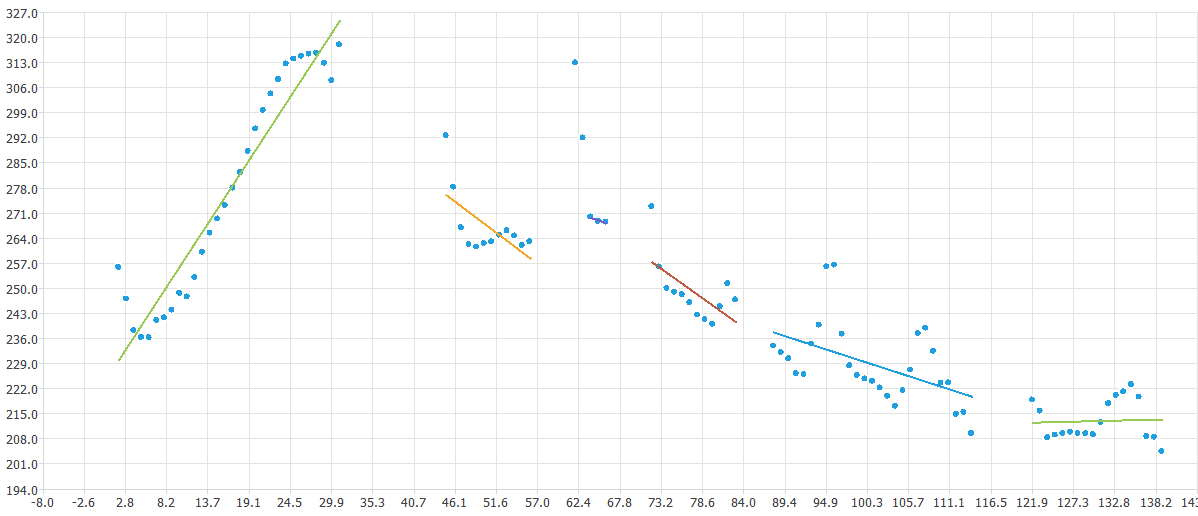
\includegraphics[scale=0.7]{rozkaz_1_kob_25.png}
\caption{Intonacja zdania rozkazującego przedstawionego na rysunku ... lecz uzyskana za pomocą PRAAT-a}
\end{figure}
\FloatBarrier

Silny nacisk położony na czasownik w trybie rozkazującym jest również odzwierciedlony w przebiegu intonacji uzyskanej za pomocą PRAAT-a. Zdanie zostało poprawnie rozpoznane przez program.

\begin{figure}[h]
\centering
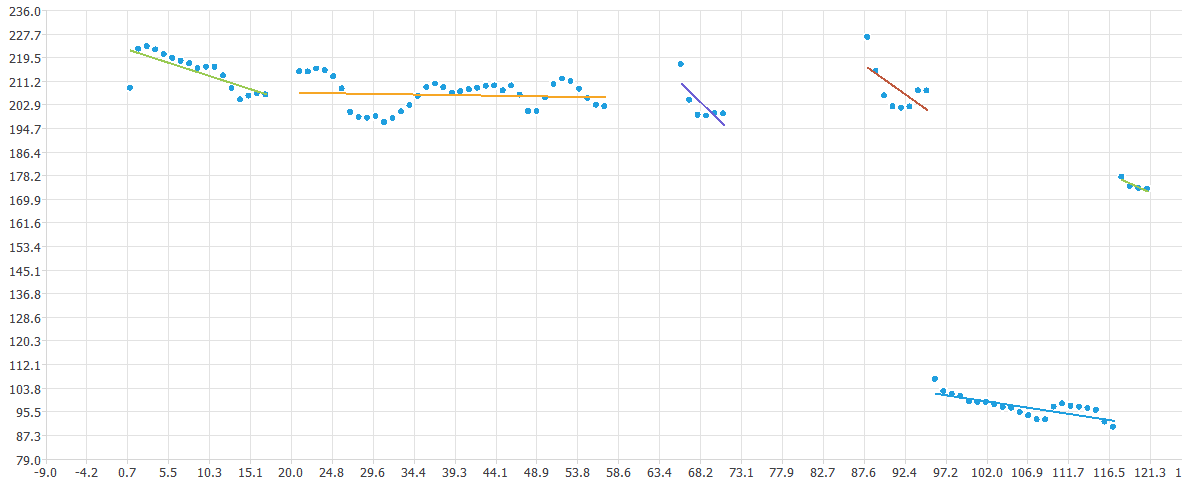
\includegraphics[scale=0.7]{tw_1_praat.png}
\caption{Intonacja zdania twierdzącego przedstawionego na rysunku ... lecz uzyskana za pomocą PRAAT-a}
\end{figure}
\FloatBarrier
Przykład zdania twierdzącego również pokazuje podobieństwo tendencji przebiegów intonacji uzyskanych w różny sposób. Stała tendencja została zachowana.
\subsection{Błędne rozpoznania}
\begin{figure}[h]
\centering
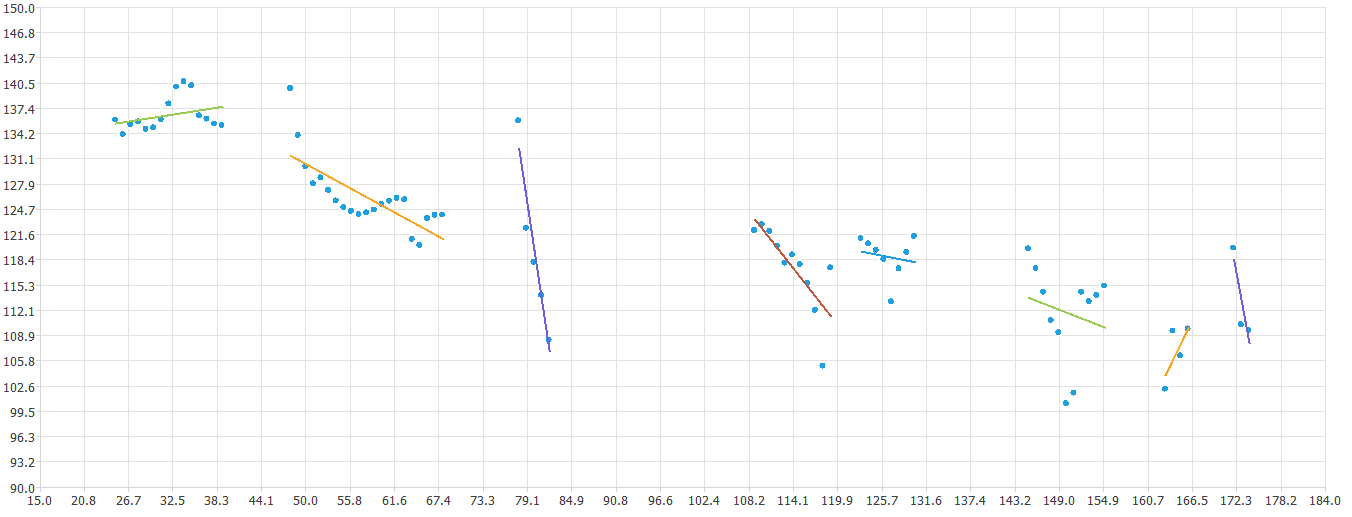
\includegraphics[scale=0.7]{rozkaz_1_praat_zle.png}
\caption{Intonacja zdania rozkazującego przedstawionego na rysunku ... lecz uzyskana za pomocą PRAAT-a}
\end{figure}
\FloatBarrier
Zdanie rozkazujące, którego intonacja uzyskana za pomocą PRAAT-a została przedstawiona na rysunku ... zostało błędnie sklasyfikowane jako zdanie twierdzące. Intonacja tego samego zdania, lecz uzyskana za pomocą YIN, została przedstawiona na rysunku ... i w tym przypadku zostało sklasyfikowane poprawnie jako zdanie rozkazujące. Przyczyn błędnego rozpoznania należy szukać w założeniach podejścia opartego na długościach segmentów oraz odległościach między nimi. W przypafku wartości uzyskiwanych za pomocą PRAAT-a zarówno segmenty jak i przerwy między nimi są stosunkowo krótsze, powodując błędy w rozpoznawaniu.
\chapter{Wnioski}
Uzyskane rezultaty można rozpatrywać dwustopniowo. Program wykorzystując algorytm YIN do esktrakcji intonacji uzyskuje bardzo dobrą skuteczność w rozpoznawaniu obu rodzajów pytań. Zaobserwowane zmiany w intonacji towarzyszącej pytaniom są wystarczające dla poprawnego rozpoznania w zdecydowanej większości przypadków. Potwierdza to dotychczasowe badania wykonane w tym zakresie. 
Trudniejszym zadaniem okazało się rozróżnianie zdań rozkazujących oraz twierdzących. Pewnym utrudnieniem była ubogość dotychczasowych badań wykonanych dla zdań rozkazujących. W toku pracy udało sie jednak zaobserwować wiele cech rózniących oba rodzaje zdań, których zastosowanie pozwoliło uzyskać zadowalające wyniki.

Opracowaną metodę opartą na zaoberwowanych cechach przetestowano również na intonacji zdań uzyskanej za pomocą innego algorytmu. Był to algorytm oparty na autokoleracji, używany przez program PRAAT.
W przypadku rozpoznawania pytań, nie zaobserwowano różnic. Rozpoznawania przebiega prawidłowo w takim samym stopniu.
Rozpoznawanie zdań rozkazujących oraz twierdzących wskazało jednak wady w podejściu opartym na długościach segmentów oraz odległościach między nimi. Uzyskane rezultaty są nieznacznie, ale jednak gorsze od tych uzyskanych bazując na ekstrakcji opartej na algorytmie YIN.

Porównanie wyników opartych na analizie intonacji uzyskanej za pomocą różnych algorytmów pokazało możliwe drogi usprawnienia metody rozpoznawania. Podejście oparte na ustaleniu wartości progowych dla długości segmentów oraz odległości między nimi okazało się dość wadliwe. Pierwszym krokiem w celu poprawy uzyskiwanych wyników powinno być zwiększenie skalowalności tego rozwiązania. Nowe podejście nie powinno używać stałych jako wartości progowych.
Kolejnym krokiem udoskonalenia metody powinno być zwiększenie bazy nagrań. Dotyczy to zwłaszcza zdań rozkazujących. Większa baza nagrań umożliwiłaby zwiększenie liczby cech odróżniających te zdania od zdań twierdzących.
\newpage

\begin{thebibliography}{99}
\bibitem{krtan}
Terapia mowy [Online] [Dostęp 05.02.2019]
http://terapiamowy.com/index.php/niedowlad-krtani/
\bibitem{speech}
Three parts of speech [Online] [Dostęp 10.02.2019]
https://uiowa.edu/voice-academy/three-parts-speech
\bibitem{mowa}
 Fernando Trujillo,The Production of Speech Sounds, English Phonetics and Phonology
\bibitem{produkcja_mowy}
Zhaoyan Zhang, Mechanics of human voice production and control [Online] [Dostęp 01.03.2019]
https://www.ncbi.nlm.nih.gov/pmc/articles/PMC5412481/

\bibitem{pros}
The prosody of speech: Melody and rythm, Sieb Nooteboom, 1997, Utrecht University
\bibitem{TS}Thornbury, Scott.:
 (2006). An A-Z of ELT. Oxford: Macmillan Publishers, Ltd.
 \bibitem{GRI-BA}
Martine Grice and Stefan Baumann, An introduction to intonation-functions and models, Ifl Phonetik and Universität Köln(2007)
\bibitem{INT-SYS}
Daniel Hirst Albert François di Cristo, A survey of intonation systems, 1998
\bibitem{SPA}
Prieto, P., and Roseano, P. (2018). Prosody: Stress, Rhythm, and Intonation. In K. Geeslin (Ed.), The Cambridge Handbook of Spanish Linguistics (Cambridge Handbooks in Language and Linguistics, pp. 211-236)
\bibitem{phonem}
Definition of phoneme, https://www.britannica.com/topic/phoneme, [Online][Dostęp 10.03.2019]
\bibitem{liczba_fonem}
Bogusław Dunaj: Dwa dyskusyjne problemy polskiej fonologii. W: Prace językoznawcze 19. Studia polonistyczne. Alina Kowalska, Aleksander Wilkoń (red.). Katowice: Uniwersytet Śląski, 1991, s. 40–46, seria: Prace Naukowe Uniwersytetu Śląskiego w Katowicach.
\bibitem{Hollien_Ship}
Hollien, H., and Ship, T. (1972) “Speaking fundamental frequency and chronological age in males,” J. Speech Hear. Res. 15, 155–159
\bibitem{Pegoraro-Krook}
Pegoraro-Krook, M. 1. (1988). “Speaking fundamental frequency characteristics of normal Swedish subjects obtained by glottal frequency analysis,” Folia Phoniatrica 40, 82–90
\bibitem{Gilbert}
Gilbert, H.R., and Weismer, G.G. (1974). “The effects of smoking on the speaking fundamental frequency of adult women,” J. Psycholing. Res. 3, 225–231. 
\bibitem{formant}
What is Formant? https://ec-concord.ied.edu.hk/phonetics\_and\_phonology/wordpress/learning\_website/chapter\_2\_vowels\_new.htm, [Online][Dostęp 10.04.2019]
\bibitem{YIN}
Kawahara H., de Cheveigne A. YIN, a fundamental frequency estimator for speech and music, 2002

\end{thebibliography}
\end{document}